
\chapter{Related works}
\label{sec:related_works}

This chapter reviews computational approaches proposed in previous works to identify driver mutations and cancer driver genes.   
Due to the scope of this work, we focus on machine learning-based solutions, discussing how interactions between data types and ML algorithms have been explored in related works. We also describe current analytical limitations identified through literature review, some of which served as motivation for the present work. The chapter is based on a survey paper published in the journal \textit{Briefings in Bioinformatics} \cite{andrades2022machine}, as follows:

\vspace{0.7cm}
\hfill\begin{minipage}{0.92\textwidth}
ANDRADES, R.; RECAMONDE-MENDOZA, M. Machine learning methods for prediction of cancer driver genes: a survey paper. \textbf{Briefings in Bioinformatics}, Volume 23, Issue 3, May 2022, bbac062. Available: \url{https://doi.org/10.1093/bib/bbac062}.
\end{minipage}


\section{Initial considerations}

Previous works have dedicated efforts to summarize and organize literature regarding computational approaches for prediction of CDGs and driver mutations, with different focuses \cite{zhang2014identifying, chen2015deciphering, cheng2016advances, dimitrakopoulos2017computational, chen2020comprehensive, Rogers+2021}.
Although some ML-based methods were covered by some of these works, they were mostly developed for a more general problem of distinguishing disease-related SNVs from common polymorphisms \cite{zhang2014identifying, chen2015deciphering}. Other surveys have categorized methods according to their major feature types \cite{cheng2016advances} or prediction strategy \cite{dimitrakopoulos2017computational}, without emphasis on ML. Recent works also focused on comparing the predictive performance of distinct computational methods for cancer drivers prediction \cite{chen2020comprehensive, pham2021computational}. Finally, \citet{Rogers+2021} reviewed generic ML-based tools to predict the pathogenic impact of human genome variants, further concentrating their discussion on a specific set of tools to predict cancer drivers.
Nonetheless, the theoretical background and methodological details of ML were not discussed by the authors.

A table summarizing the articles mentioned, with a brief description of their scope, is provided in the appendix (Table \ref{tab:relatedworks}). All these previous works, jointly, have covered a large body of the literature regarding computational methods for cancer driver discovery and have been crucial to elucidate the particular niche targeted by each solution, as well as their potential in solving the task. We emphasize, however, that aspects entailed in the development of ML models for CDG prediction were not the focus of previous discussions.
This chapter provides a comprehensive analysis of ML-based computational approaches to identify driver mutations and CDG, constructing an integrated, panoramic view of data and ML techniques within this domain. 


\section{Search methodology}


Two main bibliographic repositories were used as search sources, PubMed and DBLP. While the former is most focused on biomedical literature, the latter is specialized in computer science bibliography. These repositories were chosen because, together, they cover a wide range of papers from high-impact international scientific journals and conferences in both the fields of medicine and computer science. The query for the PubMed database was constructed using keywords related to ``cancer driver genes'', ``prediction'', and ``machine learning'' as terms of interest. For DBLP, the search was conducted using only terms related to the domain of interest since all indexed articles are within the computer science field. These terms included ``cancer driver genes'', ``cancer'', ``disease-associated genes'', and ``oncogenes''.

Our initial search returned 355 related papers found in PubMed and 84 papers retrieved from DBLP. Duplicates were removed, resulting in 420 papers. Each paper was individually evaluated regarding its relevance to the research topic covered. As inclusion criteria, we only considered papers that explicitly mention any ML algorithm as part of its methodological approach. All titles and abstracts were screened to identify papers that employed machine learning techniques to predict cancer driver genes. When necessary, we carried out a diagonal reading of the papers to confirm their suitability for this chapter’s scope. After this initial analysis, 45 (12.68\%) papers from PubMed and 7 (8.33\%) papers from DBLP were considered to be significantly related to the research question addressed by this work. Interestingly, many discarded papers focused on network-based computational methods to identify cancer drivers. Here, we only selected those that addressed the use of ML techniques in their methodology in conjunction with network-based approaches.

The 52 eligible papers were read in full for a more in-depth analysis of their methodology. We verified aspects such as which specific ML techniques were adopted in the proposed solution and the operating steps in which they were used. After this second round of paper examination, 36 papers were confirmed to be relevant, as they applied ML algorithms as a central part of the proposed computational solution for cancer drive gene prediction. Finally, to guarantee that no significant contribution to the field of cancer driver gene prediction was left behind, we manually revised the references of the selected papers to search for relevant works that our search strategy has not retrieved. Besides, we used Google Scholar to search the scientific literature for studies that have cited the selected papers and thus increase the range of articles included in this review chapter. Five papers were selected after these additional searches, totaling 41 relevant papers for our work (Table~\ref{tab:selectedPapers}). Our search was concluded on April 1st, 2021.

The acronyms used in Table~\ref{tab:selectedPapers} represent the categorization regarding the data used by the authors, Functional Genomics (FG), Functional Integration (FI), Genomic variation (GV), Ontology-based (Ob) and Network-based (Nb). As for the algorithm used, Artificial neural network (ANN), Probabilistic methods (Pm), Regression-based (Rb), SVM-based (SVM), Tree-based (Tb), Supervised learning (others) (So), Deep learning (DL), Traditional unsupervised learning (UL) and evolutionary algorithm (EA). These concepts will be explored in detail in the following sections. In addition, the performance metrics column also includes a list of acronyms used to simplify the table, accuracy (Acc), F1-measure (F1), Matthew's correlation coefficient (MCC), precision (Pre), area under the Precision-Recall curve (AUC-PR), area under the ROC curve (AUC-ROC) and recall (Rec).





%\pagebreak

\begin{landscape}

\begin{table}[!th]
\caption{Main characteristics of selected papers. \label{tab:selectedPapers}}
\centering
 \begin{adjustbox}{scale=0.7,center}
%\resizebox{\textwidth}{!}{%
\begin{tabular}{llclcll}
\hline
Reference                   & Data categories      & \multicolumn{1}{l}{Data integration} & Algorithms       & \multicolumn{1}{l}{Feature selection} & Performance metrics             & Validation strategy          \\ \hline
\citet{Carter2009}        & GV;FI          & Y                                    & Tb              & Y                                     & AUC-ROC; Acc                       & k-fold CV                       \\
\citet{Capriotti2011} & GV;FI;Ob       & Y                                    & SVM             & N                                     & AUC-ROC; Acc                        & k-fold CV                       \\
\citet{Fu2012}            & FG             & N                                    & So              & N                                     &                                 &                                 \\
\citet{Tan2012}           & GV;FI;Ob             & Y                                    & SVM             & Y                                     & Acc                             & k-fold CV                       \\
\citet{Davoli2013}        & GV;FI          & Y                                    & Rb              & Y                                     & Acc                             & k-fold CV                       \\
\citet{Mao2013}           & GV;FI          & Y                                    & SVM             & Y                                     & AUC-ROC                             & k-fold CV                       \\
\citet{Manolakos2014}     & FG;Ob             & Y                                    & UL              & N                                     &                                 & Holdout (70\%/30\%) + k-fold CV \\
\citet{Schroeder2014}     & GV;FI          & Y                                    & Rb;Tb;Pm        & N                                     & Acc                             & k-fold CV                       \\
\citet{U2014}             & FI             & N                                    & SVM;Tb;ANN;Pm;So & Y                                     & Acc; F1; Pre; Rec     & k-fold CV                       \\
\citet{Anoosha2015}       & FI          & N                                    & SVM             & Y                                     & Acc                             & k-fold CV                       \\
\citet{Gnad2015}          & GV;FI;FG       & Y                                    & Rb              & Y                                     & Acc                             & k-fold CV                       \\
\citet{Park2015}          & GV;FG;Nb       & Y                                    & Rb              & Y                                     & Acc                             &                                 \\
\citet{Soliman2015}       & GV;FI             & Y                                    & SVM;Rb          & Y                                     & Acc; F1; MCC                         & k-fold CV                       \\
\citet{Dong2016}          & GV;FI;Ob       & Y                                    & SVM;Rb          & Y                                     & AUC-ROC                             & k-fold CV                       \\
\citet{LI2016}            & GV             & N                                    & EA              & N                                     &                                 &                                 \\
\citet{Tokheim2016}       & GV;FI;FG;Nb       & Y                                    & Tb              & N                                     &                             &                                 \\
\citet{Park2017}          & GV;FG          & Y                                    & Rb              & Y                                     & Acc                             &                                 \\
\citet{Tavanaei2017}      & FI             & N                                    & DL              & N                                     & AUC-ROC; Acc; Pre; Rec     & Holdout (85\%/15\%)             \\
\citet{Agajanian2018}     & FI          & N                                    & Rb;Tb           & Y                                     & Acc; F1; Pre; Rec      & Holdout (80\%/20\%) + k-fold CV \\
\citet{Celli2018}         & FG             & N                                    & Tb              & N                                     & F1                              & Holdout (70\%/30\%)             \\
\citet{Guan2018}          & GV;FG          & Y                                    & SVM             & Y                                     &                                 & k-fold CV                       \\
\citet{Lu2018}            & GV;FG          & Y                                    & UL              & N                                     & Acc; F1; Rec                 & k-fold CV                       \\
\citet{Wang2018}          & GV;FI;FG       & Y                                    & Pm              & N                                     & AUC-ROC                             & k-fold CV                       \\
\citet{Zhou2018}          & FI;Ob;Nb    & Y                                    & Tb              & Y                                     & F1; Rec; MCC                     & k-fold CV                       \\
\citet{Agajanian2019}     & GV;FI          & Y                                    & Tb;DL           & Y                                     & AUC-ROC; Acc; F1                    & Holdout (80\%/20\%) + k-fold CV \\
\citet{Althubaiti2019}    & Ob             & N                                    & ANN              & N                                     & AUC-ROC; F1                         & k-fold CV                       \\
\citet{Collier2019}       & GV;FI;Nb          & Y                                    & SVM             & N                                     & AUC-ROC                             & k-fold CV                       \\
\citet{Han2019}           & GV             & N                                    & So              & N                                     &                                 &                                 \\
\citet{Jiang2019}         & GV;FG          & Y                                    & Tb              & N                                     &                            &                                 \\
\citet{Luo2019}           & GV;FG          & Y                                    & DL              & N                                     & AUC-ROC                             &                                 \\
\citet{Nicora2019}       & GV;FI          & Y                                    & SVM;Rb;Tb       & N                                     & Acc; Rec                     & Holdout (70\%/30\%) + k-fold CV \\
\citet{Schulte-Sasse2019} & GV;FG;Nb       & Y                                    & DL              & N                                     & AUC-ROC; AUC-PR; MCC                   & k-fold CV                       \\
\citet{Xi2019}            & GV             & N                                    & UL              & N                                     & Pre; Rec               & k-fold CV                       \\
\citet{Zhu2019}           & FI             & N                                    & -         & N                                     &                                 &                                 \\
\citet{Chandrashekar2020} & GV;FI             & Y                                    & Tb              & N                                     & Acc                             & k-fold CV                       \\
\citet{Colaprico2020}     & GV;FI;FG;Ob;Nb       & Y                                    & Tb              & N                                     &                                 &                                 \\
\citet{Cutigi2020}        & GV;Nb          & Y                                    & SVM;Tb          & N                                     & AUC-ROC; Acc; F1; Pre; Rec & k-fold CV                       \\
\citet{Gumpinger2020}     & FI;Nb             & Y                                    & SVM;Rb;Tb       & N                                     & F1; Pre; Rec; AUC-PR  & k-fold CV                       \\
\citet{Lyu2020}           & GV;FI;FG;Ob    & Y                                    & SVM;Rb;Tb       & Y                                     & Acc; Pre; Rec; AUC-PR & k-fold CV                       \\
\citet{Wang2020}           & FI    & N                                    & SVM;Tb;ANN;So       & N                                     & AUC-ROC; Acc; F1; Pre; Rec & k-fold CV                       \\
\citet{Nulsen2021}        & GV;FI;FG;Ob;Nb & Y                                    & SVM             & Y                                     & AUC-ROC                             & k-fold CV                       \\ \hline

\end{tabular}%
%}
\end{adjustbox}
%\begin{tablenotes}%
%\item[$^{1}$] FG: Functional Genomics; FI: Functional Integration; GV: Genomic variation; Ob: Ontology-based; Nb: Network-based.
%\item[$^{2}$] ANN: Artificial neural network; Pm: Probabilistic methods; Rb: Regression-based; SVM: SVM-based; Tb: Tree-based;  So: Supervised learning (others); DL: Deep learning; UL: Traditional unsupervised learning; EA: evolutionary algorithm.
%\item[$^{3}$] Acc: accuracy; F1: F1-measure; MCC: Matthew's correlation coefficient; Pre: precision; AUC-PR: area under the Precision-Recall curve; AUC-ROC: area under the ROC curve; Rec: recall.  
%\end{tablenotes}

\end{table}
\end{landscape}



\section{Overview of selected papers}

Papers distribution according to the publication year (Figure~\ref{fig:papers-year}) suggests a growing interest in the research topic. Most papers (56.09\%) were published after 2018 and the highest number of publications were found in 2019 (10). The low number of related papers published in 2021 is justified by the short period covered by our analysis. Papers were published mainly in scientific journals, with only five \cite{Fu2012, Tavanaei2017, Nicora2019, Schulte-Sasse2019, Cutigi2020} appearing in conference proceedings. The top three journals in terms of number of papers were Bioinformatics (6), Journal of Computational Biology (3), and Plos One (3).

\begin{figure}[!h]
    \centering
    \caption{Number of selected papers per year of publication.}
    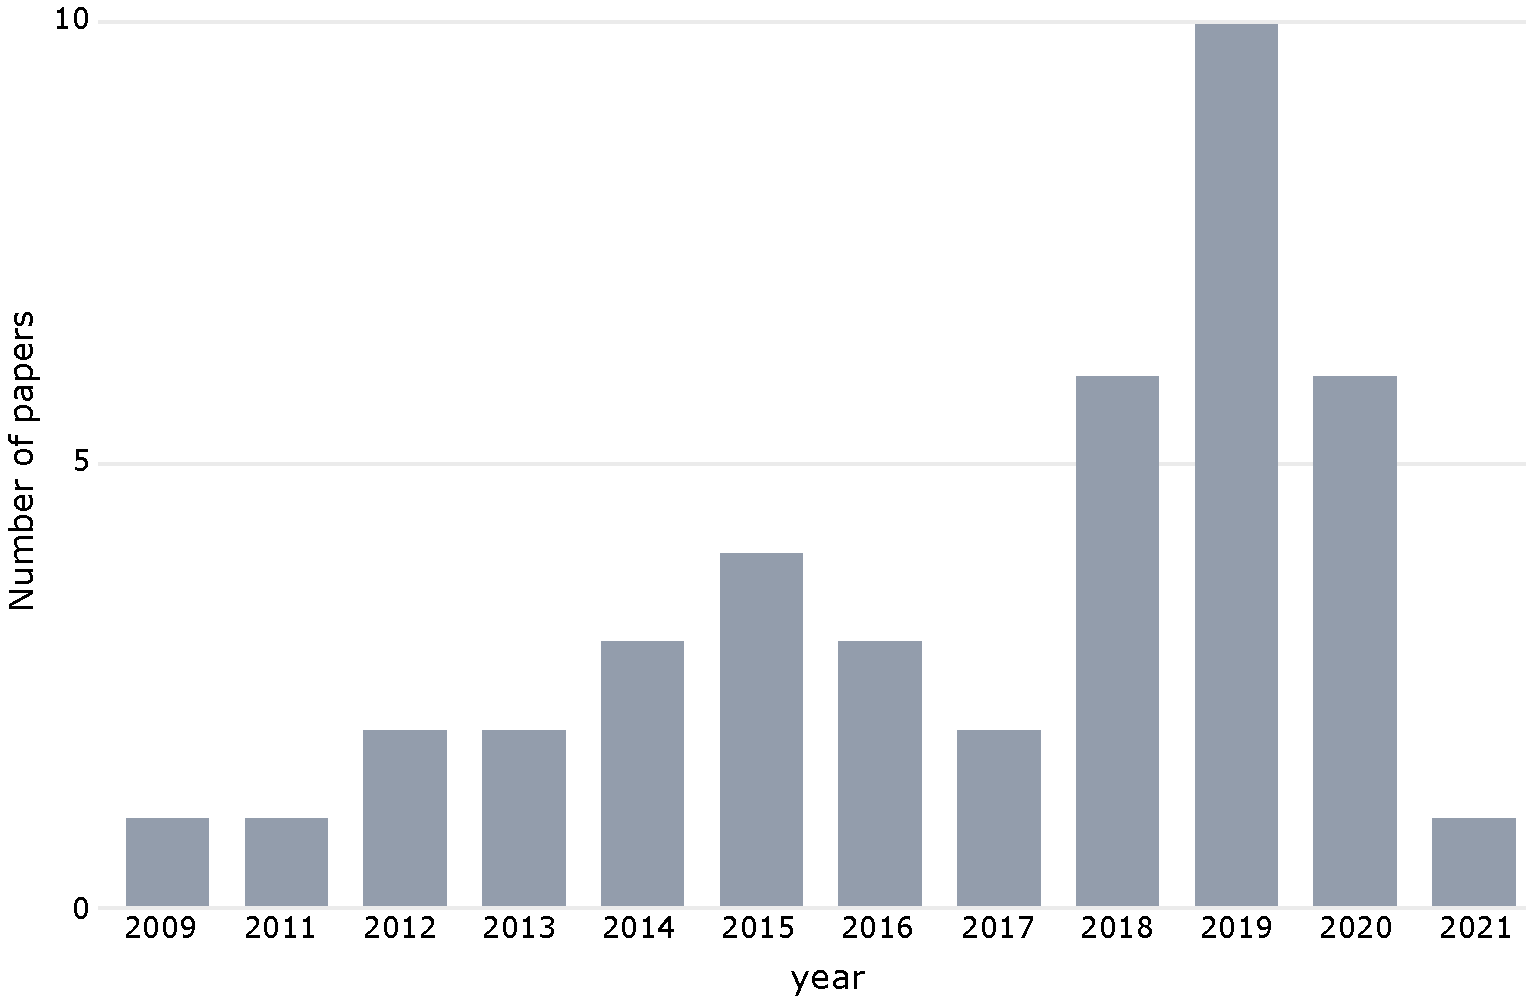
\includegraphics[width=0.90\textwidth]{images/survey/Figure1_Papers_x_year.pdf}
    \legend{Source: Prepared by the author}
    \label{fig:papers-year}
\end{figure}

In terms of target prediction problem, 32 papers (\ie 78.04\%) concentrated in running predictions at the gene level. Among these, six papers \cite{Davoli2013, Gnad2015, Tavanaei2017, Chandrashekar2020, Colaprico2020, Lyu2020} aimed to distinguish oncogene and tumor suppressor gene (TSG) (\ie the two subclasses of CDGs), whereas the others focused on classifying a given gene as CDG or not. Seven papers targeted predictions on mutation level \cite{Mao2013, U2014, Soliman2015, Agajanian2018, Zhou2018, Agajanian2019, Wang2020}, most of which restricted the analysis for missense mutations. We also found one paper aiming at identifying cancer modules to discover cancer driver genes \cite{Manolakos2014} and other focusing on the prediction of false positive CDGs \cite{Cutigi2020}. Also, while most papers addressed cancer drivers in general, some focused on specific types of cancer, such as colon adenocarcinoma \cite{Fu2012, Luo2019}, breast cancer \cite{Celli2018, Lu2018, Luo2019}, lung adenocarcinoma \cite{Luo2019}, thyroid \cite{Celli2018}, and kidney \cite{Celli2018}. We also observed predictive models for cancer-related mutations in human protein kinases \cite{U2014} and, more specifically, in the Epidermal Growth Factor Receptor \cite{Anoosha2015}.

To better map the current state-of-the-art in terms of available resources and adopted methodologies, two main analyses were made. The first one focused on the data types used as model's feature, while the second focused on summarizing the computational aspects of the proposed predictive model, such as type of learning and specific ML algorithms adopted. The next sections describe and organize the selected papers in terms of data categories and computational strategies.


\section{Data categories}

A core component for ML-based predictive models is the training data due to the common sense that much of the model's success depends on the fed data. A given prediction problem may have its concept represented in many different ways, which is especially true in the genomics domain. Some of these representations may be better than others in revealing the patterns we sought to learn. Thus, a clear comprehension of the possible types of features for instances representation within our domain may provide insights into current limitations and new analytical opportunities.
We observed a large variety of information used as models' input features for cancer drivers prediction. After careful analysis of the selected papers, we classified them into five categories based on the properties evaluated as predictors (Table \ref{tab:features}): (1) \textit{Genomic Variation} (GV), (2) \textit{Functional Impact} (FI), (3) \textit{Functional Genomics} (FG), (4) \textit{Network-based} (Nb), and (5) \textit{Ontology-based} (Ob). Subcategories were defined for some categories to better organize the corresponding features based on their semantics.

\begin{table*}[!ht]
\caption{Data categories and subcategories adopted to classify selected papers according to types of features employed.\label{tab:features}}
\centering
\resizebox{\textwidth}{!}{%
\begin{tabular}{L{3cm}L{3.5cm}L{15cm}}
\hline
\multicolumn{1}{c}{Category}                           & \multicolumn{1}{c}{Subcategory} & \multicolumn{1}{c}{Description}                                                          \\ \hline
\multicolumn{1}{c}{\multirow{3}{*}{Genomic Variation}} & Mutations                       & properties of somatic single nucleotide variants (SNV) and frameshift insertion/deletion (\eg estimate of the mutation frequency, mutation ratio, mutation hotspots) \\ \cline{2-3} 
\multicolumn{1}{c}{}                                   & Copy number alteration (CNA)    & information related to amplifications, deletions, and duplication of segments of DNA that changes the number of copies of a particular DNA segment within the genome (\eg deletion and amplification frequency)                                      
\\ \cline{2-3} 
\multicolumn{1}{c}{}                                   & DNA sequence                    & raw nucleotide sequence                                                                  \\ \hline
\multirow{3}{*}{Functional Impact}                     & Functional impact scores        & outputs of \textit{in silico} variant effect predictors concerning the probability of deleterious changes on protein function                                            \\ \cline{2-3} 
                                                       & Protein-based                   & properties of protein sequence and structure, from amino acids to protein's tertiary structure      \\ \cline{2-3} 
                                                       & Evolution-based                 & evolutionary conservation scores, amino acids substitution rate, gene age, gene damage index, number of human paralogs, etc.                                             \\ \hline
\multirow{3}{*}{Functional Genomics}                   & Transcriptomics                 & large-scale gene expression profiles or statistics  derived  from  differential gene expression analyses   \\ \cline{2-3} 
                                                       & Epigenomics                     & DNA methylation, histone modifications, chromatin accessibility, DNA replication time    \\ \cline{2-3} 
                                                       & Proteomics                      & protein expression data, mainly expressed as categorical features that indicate whether or not a protein is expressed in a given human tissue                                                            \\ \hline
Ontology-based                                         & -                               & functional, cellular, or phenotypic annotations obtained from bioinformatics databases or related works                                                  \\ \hline
Network-based                                          & -                               & node properties from structural analysis of molecular networks (\eg PPI or gene-gene networks)         \\ \hline
\end{tabular}%
}
\end{table*}

A general overview of papers in terms of the data categories employed is shown in Figure~\ref{fig:DataCategories}. \textit{Genomic variation} was the most common feature category used (29 papers, \ie 70.73\%), followed by \textit{Functional Impact} (26 papers) and \textit{Functional Genomics} (16 papers). \textit{Network-based} and \textit{Ontology-based} features were each employed in 9 papers (Figure~\ref{fig:DataCategories_a}). Since some data categories contain multiple subcategories, we analyzed the number of distinct feature datasets adopted per paper and found that it varied from 1 to 8 (\cite{Nulsen2021}), with an average of 2.87 ($\pm$ 1.17) datasets. 


\begin{figure*}[!ht]
\centering

\caption{Analysis of data categories used as model features by selected papers.}

\subfloat[Relation of data categories per paper, organized by year of publication in ascending order. \label{fig:DataCategories_a}]{%
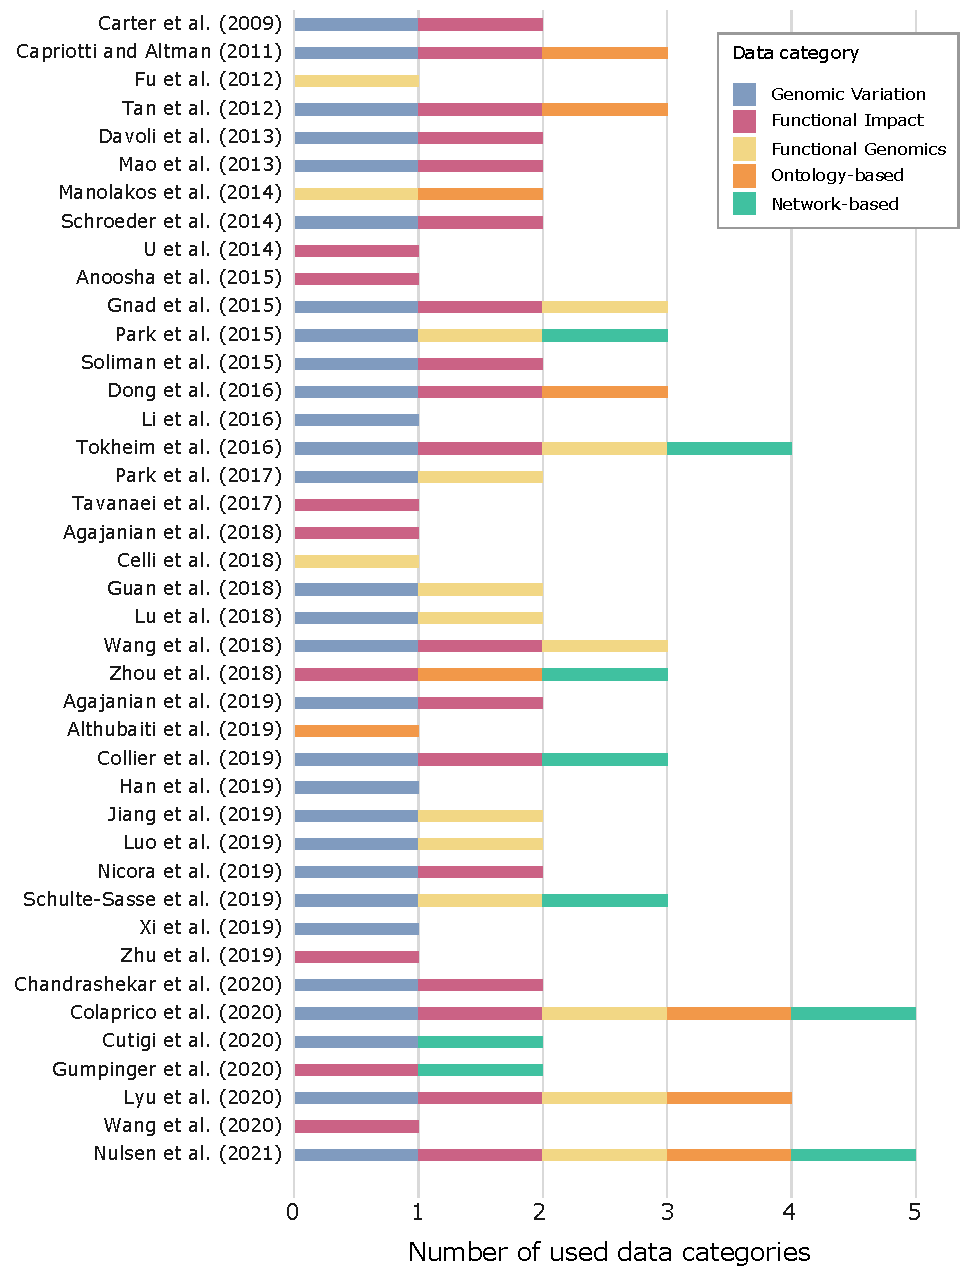
\includegraphics[width=0.65\textwidth]{images/testes/Figure2_DataCategories_a.pdf}}
\hspace{\fill}
\subfloat[Distribution observed in the use of the data categories per year of publication. \label{fig:DataCategories_b} ]{%
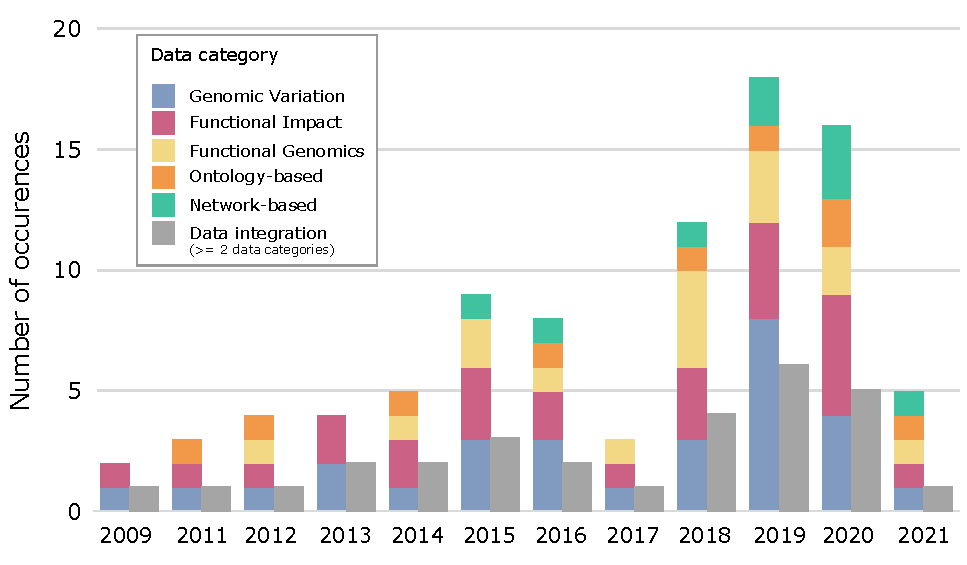
\includegraphics[width=0.59\textwidth]{images/testes/Figure2_DataCategories_b.pdf}}
\hspace{\fill}
\subfloat[Venn diagram showing the intersection of studies in terms of employed data categories. \label{fig:DataCategories_c}]{%
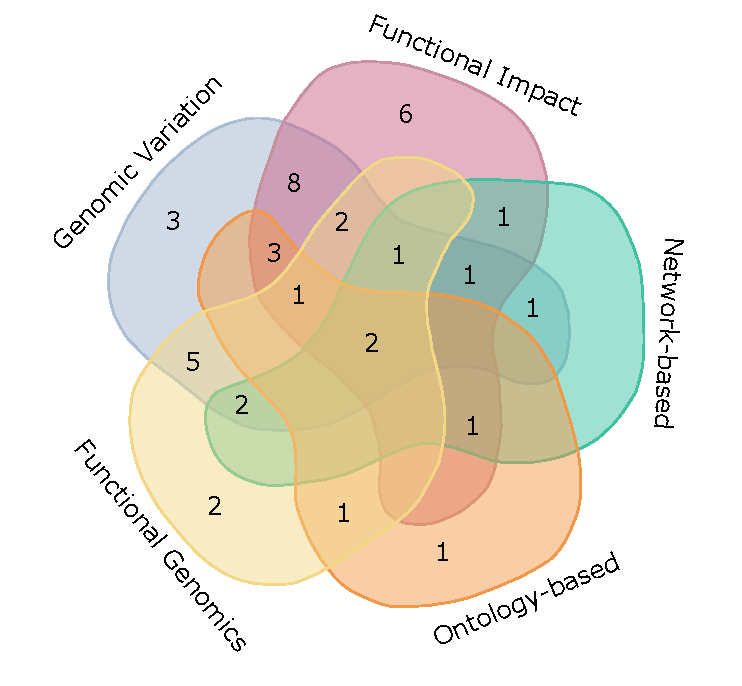
\includegraphics[width=0.40\textwidth]{images/testes/Figure2_DataCategories_c.pdf}}\\
\legend{Source: Prepared by the author}
\label{fig:DataCategories}
\end{figure*}


One of our main findings regarding the features aspect of ML models is that many works adopted more than one data category. Twenty-nine papers (\ie 70.73\%) used two or more data categories and were classified in a \textit{Data integration} category. The distribution of the number of occurrences of data categories by years of publication does not suggest any association between these factors (Figure~\ref{fig:DataCategories_b}). 
 
\begin{comment}
\begin{figure*}[!ht]
\centering
\caption{Analysis of data categories used as model features by selected papers.  (a) Relation of data categories per paper, organized by year of publication in ascending order. (b) Distribution observed in the use of the data categories per year of publication. (c) Venn diagram showing the intersection of studies in terms of employed data categories.}
\sbox{\measurebox}{%
  \begin{minipage}[b]{.47\textwidth}
  \subfloat
    []
    {\label{fig:DataCategories_a}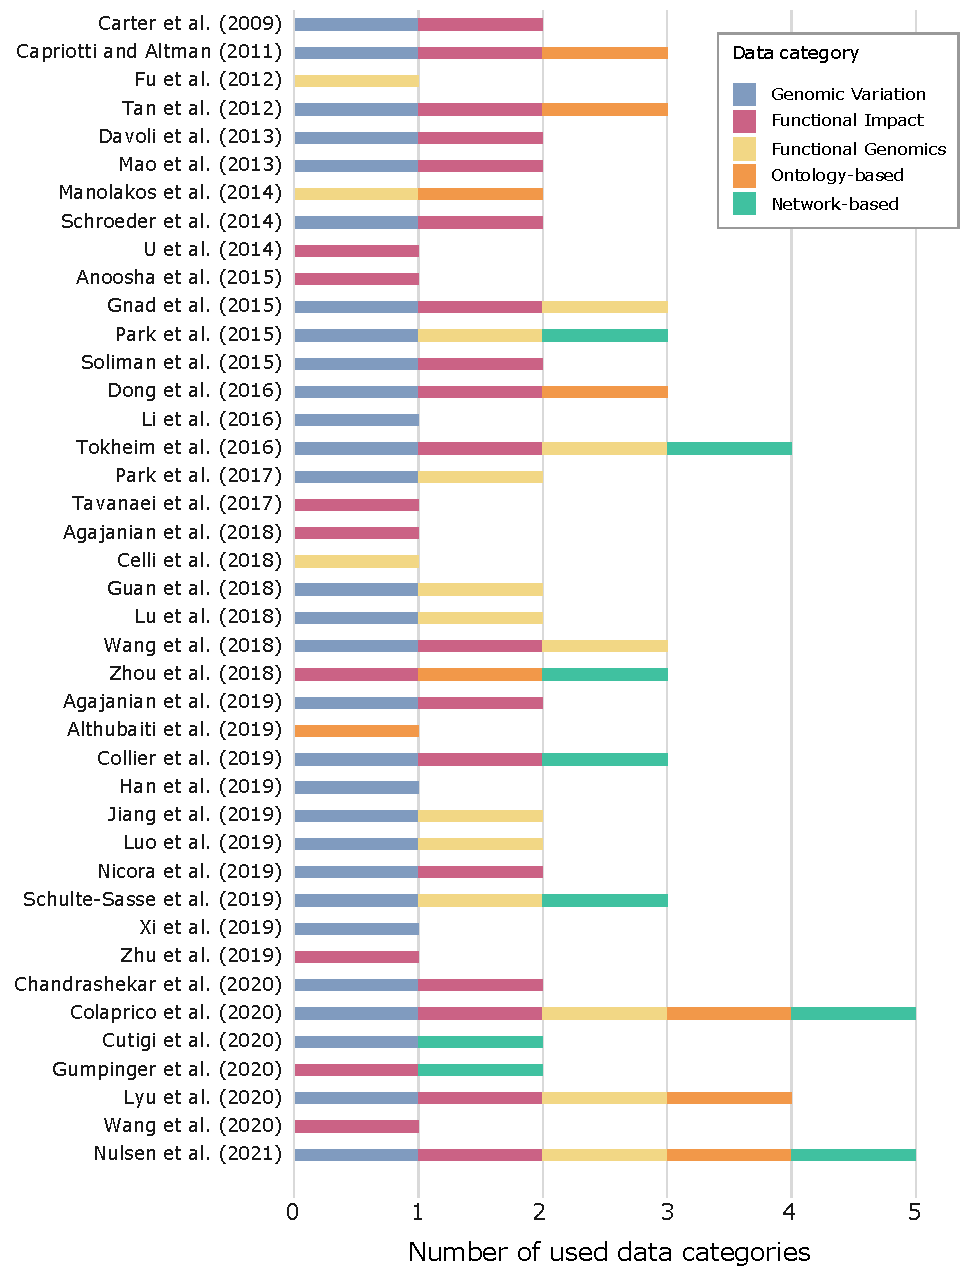
\includegraphics[width=\textwidth]{images/testes/Figure2_DataCategories_a.pdf}}
  \end{minipage}}
  
\usebox{\measurebox}\qquad
\begin{minipage}[b][\ht\measurebox][s]{.47\textwidth}
\centering
\subfloat
  []
  {\label{fig:DataCategories_b}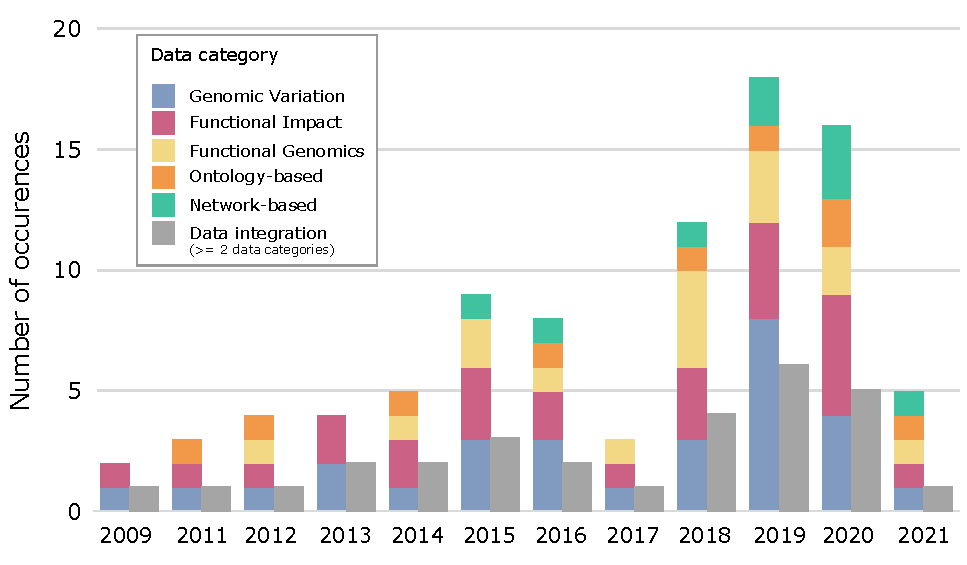
\includegraphics[width=0.9\textwidth]{images/testes/Figure2_DataCategories_b.pdf}}

\vfill

\subfloat
  []
{\label{fig:DataCategories_c}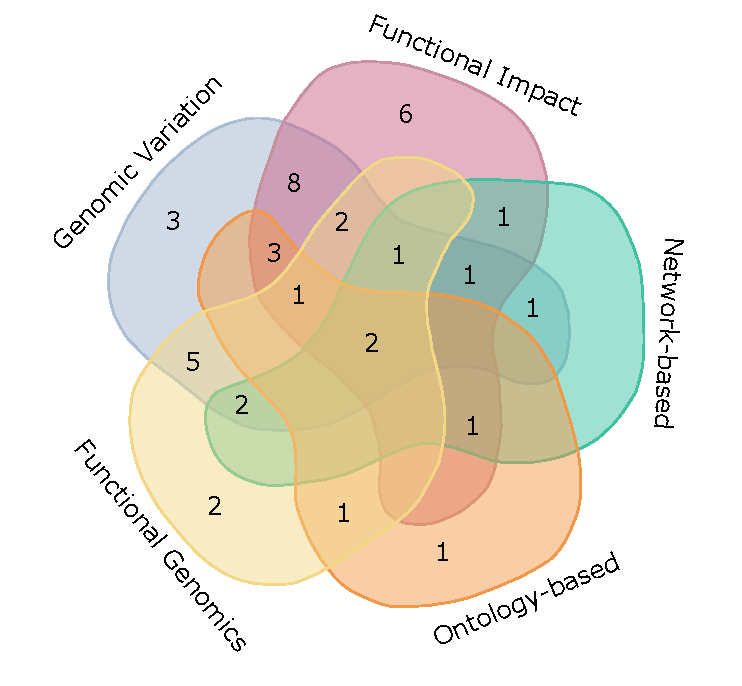
\includegraphics[width=0.73\textwidth]{images/testes/Figure2_DataCategories_c.pdf}}
\end{minipage}
\legend{Source: Prepared by the author}
\label{fig:DataCategories}
\end{figure*}
\end{comment}

Moreover, integrating different data categories is not necessarily a recent tendency, as papers published in 2009 and 2011 already proposed such strategy. Nonetheless, most of the papers using features from three or more data categories were published from 2015, and those that used four \cite{Tokheim2016, Lyu2020} or five \cite{Colaprico2020, Nulsen2021} data categories were published mainly in 2020 and 2021, which may indicate a trend for increasing data diversity in newer models. 

The Venn diagram in Figure~\ref{fig:DataCategories_c} summarizes the intersections among distinct data categories. The most recurrent combination was the integration of \textit{Genomic Variation} and \textit{Functional Impact} (8 papers), followed by \textit{Genomic Variation} and \textit{Functional Genomics} (5 papers). Also, while \textit{Functional Impact} was the most common data category used as a single source of features in the proposed models, the \textit{Network-based} category was not exclusively used by any ML model among the revised papers. In what follows, we 
review the particularities of each data category. 


\subsection{Genomic variation}

Three papers \cite{LI2016, Han2019, Xi2019} used \textit{Genomic Variation} data as the single source of feature, whereas 23 (\ie 56.09\%) combined it with other categories. A long-standing hypothesis in the discovery of cancer drivers is that driver genes are mutated more frequently than expected as compared to a background mutation rate (BMR) estimated from cancer samples for a given cancer type \cite{tamborero2013comprehensive}. Nonetheless, the mutational landscape of cancer consists of `mountains' of very frequently mutated genes and of `hills' of significantly but less frequently mutated genes \cite{vogelstein2013cancer}. Thus, simply characterizing candidate driver genes with frequency-based methods poses the challenge of robust BMR estimation: a low BMR may lead to many spurious findings, whereas a high BMR may miss the driver genes mutated at very low frequency. ML-based methods aim to allow the algorithm to learn the mutational patterns related to cancer drivers from training data. 
Here, we considered three subcategories (Table~\ref{tab:features}): i) mutations, 
ii) copy number alteration (CNA); 
and iii) raw DNA sequence, which was included since information regarding DNA variants would be implicitly available.

Mutation-related properties was the most common feature type, employed by 26 papers (\ie 63.41\%). Fifteen papers explored mutations' properties as the single source of genomic variation features, and one paper \cite{Han2019} exclusively relied on mutation-based features for model development. Mutation frequency was widely used by selected papers, usually estimated from databases such as Catalogue of somatic mutations in cancer (COSMIC)  \cite{cosmic}, The Cancer Genome Atlas (TCGA), and HapMap \cite{hapmap}. Some works \cite{Davoli2013, Gnad2015, Lyu2020} distinguished between potentially high (HiFI) or low (LoFI) functional impact mutations when computing mutation frequency, adopting \textit{in silico} predictors 
of mutations' functional impact. Moreover, silent mutations and LoFI missense mutations, or a combination of both \cite{Gnad2015,Lyu2020}, were often taken as a measure for genes' BMR. 
\citet{Davoli2013} proposed an entropy-based mutation selection score that reflects the spatial distribution of these features, measuring the occurrence of `mutation hotspots'. This measure of positional clustering was adopted by several papers \cite{Gnad2015, Tokheim2016, Collier2019, Luo2019, Colaprico2020, Nulsen2021}. Mutation hotspots were also detected using scores computed by OncoDriveCLUST \cite{tamborero2013oncodriveclust, Schroeder2014, Nulsen2021} and applying density estimates to aggregate closely-spaced missense mutations into peaks and compute mutation fraction inside the highest peak \cite{Chandrashekar2020}.

The normalized number of single nucleotide variants (SNVs) in the mutation's exon \cite{Mao2013}, mutations' distance to closest Transcribed Sequence Start (TSS) and closest Transcribed Sequence End (TSE) \cite{Agajanian2019}, and a gene-level binary matrix summarizing mutation occurrence across all samples \cite{LI2016,Xi2019} were also adopted. 

Fourteen papers (\ie 34.15\%) \cite{Davoli2013, Schroeder2014, Gnad2015, Park2015, Dong2016, LI2016, Park2017, Guan2018, Lu2018, Jiang2019, Schulte-Sasse2019, Xi2019, Lyu2020, Nulsen2021} adopted CNA data as models' features, which was first introduced in this domain by \citet{Davoli2013}. 

Their model analyzed the deletion and amplification frequency to distinguish among neutral genes, oncogenes, and TSGs.
Two papers \cite{Gnad2015, LI2016} employed the Genomic Identification of Significant Targets In Cancer (GISTIC) \cite{gistic, gistic2} algorithm to obtain DNA amplification and deletion regions. 
\citet{Gnad2015} used as features the sums of amplification or deletion frequencies across 13 TCGA cancer types. Eleven papers that fall within the CNA subcategory also adopted mutation data. However, in most cases, the features from the different subcategories were used independently rather than combined into a single input feature. One exception is the work by \citet{Schulte-Sasse2019}, in which the sum of SNVs and CNA is averaged across all samples of a given cancer type to estimate a cancer mutation rate per gene. Furthermore, among the three papers that apply only CNA features from the \textit{Genomic variation} category, two \cite{Park2017, Guan2018} also adopted gene expression data in their analyses, since CNA is known to mediate phenotypic changes through their impact on expression. \citet{Park2017} quantified the association between CNA and gene expression using a previously proposed method \cite{yuan2011sparse}, differentiating between cis-effects (\ie when gene expression is influenced by CNA in proximal genes within a several Mb window) and trans-effects (\ie  when gene expression is influenced by remote alterations throughout the genome). \citet{Guan2018} used gene-level summarized cell-lines CNA and expression profiles obtained from the Cancer Cell Line Encyclopedia (CCLE). 

Finally, only one paper \cite{Agajanian2019} used raw DNA sequence as model's features. Mutations were represented by stacking two nucleotide sequences on top of each other, one with the original nucleotide for a given position and the other with the mutated version, and a convolutional neural network (CNN) was trained to automatically extract driver-related sequence patterns. 


\subsection{Functional impact}

The functional impact (FI) of SNVs on protein function was analyzed by 63.41\% of papers. Their goal is to better identify lowly recurrent mutated driver genes or driver genes that are mutated late during tumor development, which are more challenging cases for methods that exclusively analyze genomic variation features \cite{Oncodrive-fm}. This has become a widely applied strategy even outside the scope of ML-based papers, as reflected by the several computational methods developed for pathogenicity prediction of SNVs \cite{chen2020comprehensive, wu2016dbwgfp}. 
Three subcategories were created (Table~\ref{tab:features}): i) functional impact scores provided by \textit{in silico} predictors for variant effect;
ii) protein-based features; 
and iii) evolution-based features. 
Although most FI predictors rely on features related to proteins' properties or evolutionary conservation \cite{chen2020comprehensive}, we did not consider this in our classification. 

FI scores was the largest subcategory, employed by 18 papers. Table~\ref{tab:fi_tools} summarizes the FI predictors used. Most works adopted the predicted scores or p-values as models' features, while others (\eg \cite{Collier2019}) estimated the number of damaging missense mutations per gene using a pre-defined score threshold. Several works integrated the output of multiple FI predictors in their feature vectors \cite{Mao2013, Dong2016, Agajanian2018, Agajanian2019, Zhu2019, Wang2020}. \citet{Dong2016} used 11 tools for point coding mutations and one tool, FunSeq2 \cite{funseq2}, to annotate non-coding variants. 
\citet{Wang2020} explored the largest diversity of tools: 23 conservation-base, ensemble-based, and function-prediction methods.

\begin{table*}[!th]
\caption{\textit{In silico} tools for functional impact prediction \label{tab:fi_tools}}
\centering
\resizebox{\textwidth}{!}{%
\begin{tabular}{L{4.7cm}L{17cm}}
\hline
\textbf{Reference} & \textbf{Tools} \\ \hline
\citet{Capriotti2011} & PANTHER \cite{panther} \\ \hline
\citet{Davoli2013}  & Polyphen-2 \cite{PolyPhen-2}\\ \hline
\citet{Mao2013} & SIFT \cite{ng2003sift}, PolyPhen-2 \cite{PolyPhen-2}, CONDEL \cite{condel}, MutationAssessor \cite{MutationAssessor}, PhyloP \cite{PhyloP}, GERP++ \cite{GERP++}, and LRT \cite{LRT} \\ \hline
\citet{Schroeder2014}  & OncodriveFM \cite{Oncodrive-fm}\\ \hline
\citet{Gnad2015} & MutationAssessor \cite{MutationAssessor} \\ \hline
\citet{Dong2016}  & SIFT \cite{ng2003sift}, PolyPhen-2 \cite{PolyPhen-2}, LRT \cite{LRT}, MutationTaster \cite{schwarz2010mutationtaster}, MutationAssessor \cite{MutationAssessor}, FATHMM \cite{shihab2013predicting}, GERP++ \cite{GERP++}, PhyloP \cite{PhyloP}, CADD \cite{kircher2014general}, VEST \cite{carter2013identifying}, SiPhy \cite{garber2009identifying}, FunSeq2 \cite{funseq2}\\ \hline
\citet{Tokheim2016} & VEST \cite{carter2013identifying} \\ \hline
\citet{Agajanian2018}  & SIFT \cite{ng2003sift}, PolyPhen-2 \cite{PolyPhen-2}, LRT \cite{LRT}, MutationAssessor \cite{MutationAssessor}, MutationTaster \cite{schwarz2010mutationtaster}, FATHMM \cite{shihab2013predicting}, MSRV \cite{jiang2007sequence}, SinBaD \cite{lehmann2013exploring}, GERP++ \cite{GERP++}, SiPhy \cite{garber2009identifying}, PhyloP \cite{PhyloP}, Grantham \cite{grantham1974amino}, CADD \cite{kircher2014general}, GWAVA \cite{ritchie2014functional}, MetaLR \cite{dong2015comparison}, and MetaSVM \cite{dong2015comparison}\\ \hline
\citet{Wang2018}  & SIFT \cite{ng2003sift} and GERP++ \cite{GERP++} \\ \hline
\citet{Zhou2018}   & ENTPRISE \cite{zhou2016entprise}  \\ \hline
\citet{Agajanian2019} & SIFT \cite{ng2003sift}, PolyPhen-2 \cite{PolyPhen-2}, LRT \cite{LRT}, MutationAssessor \cite{MutationAssessor}, MutationTaster \cite{schwarz2010mutationtaster}, FATHMM \cite{shihab2013predicting}, MSRV \cite{jiang2007sequence}, SinBaD \cite{lehmann2013exploring}, GERP++ \cite{GERP++}, SiPhy \cite{garber2009identifying}, PhyloP \cite{PhyloP}, Grantham \cite{grantham1974amino}, CADD \cite{kircher2014general}, GWAVA \cite{ritchie2014functional}, MetaLR \cite{dong2015comparison}, and MetaSVM \cite{dong2015comparison}\\ \hline
\citet{Collier2019} & Polyphen-2 \cite{PolyPhen-2}\\ \hline
\citet{Zhu2019} & 20/20+ \cite{Tokheim2016}, MutSigCV \cite{lawrence2013mutational}, OncodriveFM \cite{Oncodrive-fm}, OncodriveCLUST  \cite{tamborero2013oncodriveclust}, DrGaP \cite{hua2013drgap}, and MUFFINN \cite{cho2016muffinn}\\ \hline
\citet{Colaprico2020}  & VEST \cite{carter2013identifying} \\ \hline
\citet{Gumpinger2020} & MutsigCV  \cite{lawrence2013mutational} \\ \hline
\citet{Lyu2020}  & VEST \cite{carter2013identifying}, PolyPhen-2 \cite{PolyPhen-2}\\ \hline
\citet{Wang2020} & GERP++ \cite{GERP++}, PhastCons, PhyloP \cite{PhyloP}, LRT \cite{LRT}, SiPhy \cite{garber2009identifying}, FATHMM \cite{shihab2013predicting}, fitCons \cite{gulko2015method}, MutationAssessor \cite{MutationAssessor}, MutationTaster \cite{schwarz2010mutationtaster}, PolyPhen2-HDIV \cite{PolyPhen-2}, PolyPhen2-HVAR \cite{PolyPhen-2}, PROVEAN \cite{choi2015provean}, SIFT \cite{ng2003sift}, VEST3 \cite{carter2013identifying}, CADD \cite{kircher2014general}, DANN \cite{quang2015dann}, Eigen \cite{ionita2016spectral}, FATHMM-MKL \cite{shihab2015integrative}, GenoCanyon \cite{lu2015statistical}, M-CAP \cite{jagadeesh2016m}, MetaLR \cite{dong2015comparison}, MetaSVM \cite{dong2015comparison}, and REVEL \cite{ioannidis2016revel} \\ \hline
\end{tabular}%
}
\end{table*}

The protein-based subcategory was adopted by 11 papers. Some works \cite{Carter2009, Tan2012, Mao2013} evaluated the changes in residues' charge, volume, polarity, the hydrophobicity resulting from the mutation, the predicted residue solvent accessibility and backbone flexibility, the mutation's effect on protein stability, and the probability that the secondary structure of the wild type residue's region is helix, loop, or strand. \citet{Anoosha2015} considered 49 physical, chemical, energetic, and conformational parameters comparing wild type and mutant residues, as well as neighboring residue information at different window lengths. Feature vectors encoding the mutated sequence and the mutation's local sequence environment \cite{Capriotti2011} or the biochemical properties of the atomic coordinates of proteins' PDB structure \cite{Tavanaei2017} were also proposed. Other characteristics considered were the fraction of the affected protein structure \cite{Zhou2018}, amino acid composition of the residues in contact with the mutation or of its domain \cite{Zhou2018}, amino acid's position in the codon or protein \cite{Agajanian2019}, number of complexes containing the protein \cite{Nulsen2021}, and background probability for observing the wild type or mutant residue in the first, middle, or last position of an amino acid triple, or at the center of a window of 5 amino-acid residues \cite{Carter2009, Tan2012}. Finally, amino acids substitution scores were employed by several studies \cite{Carter2009, Tan2012, Mao2013, U2014, Anoosha2015}, most of which integrated distinct substitution scoring matrices. 


The evolution-based subcategory was employed in 14 studies, most of which computed evolutionary conservation scores using distinct strategies or tools \cite{Carter2009, Capriotti2011, Mao2013, U2014, Anoosha2015, Tokheim2016, Agajanian2018, Zhou2018, Agajanian2019, Colaprico2020, Lyu2020}. MGAentropy, for instance, was employed by three papers \cite{Mao2013,Tokheim2016, Lyu2020}. The rationale is that the more an amino-acid residue is functionally or structurally important, the more conserved is over evolution. \citet{Chandrashekar2020} computed the mean substitution rate of all protein's positions as well as of positions under the highest peak of closely-spaced mutations. \citet{Lyu2020} employed the gene age, gene damage index, and the number of human paralogs for each gene, among others. Finally, \citet{Nulsen2021} included the indication of genes' evolutionary origin (\ie pre-metazoan, metazoan, vertebrate, or post-vertebrate).

We observed that six studies \cite{U2014, Anoosha2015, Tavanaei2017, Agajanian2018, Zhu2019, Wang2020} in the \textit{Functional Impact} category only used this data type for developing their predictive models (Figure~\ref{fig:DataCategories_a}). Among these, \citet{Zhu2019} and \citet{Wang2020} defined their features exclusively based on scores from FI predictors. This is not surprising, as this feature carries rich underlying information provided by the various properties analyzed by each FI predictor. 

\subsection{Functional genomics}

About 39\% of papers used \textit{Functional Genomics} features, which we divided in three subcategories (Table~\ref{tab:features}): i) transcriptomics; ii) epigenomics; and iii) proteomics. The motivation comes from the observation that mutation frequency is strongly correlated with transcriptional activity and DNA replication timing \cite{Jiang2019, lawrence2013mutational}, and that driver gene mutations are tightly tied to DNA methylation landscape in multiple types of cancer \cite{chen2017significant}. Moreover, mutation rates vary among individual genes and are influenced by many factors, including the chromatin state \cite{schuster2012chromatin} and the aforementioned ones (\ie gene expression, replication timing, DNA methylation). Thus, integrating these properties in the ML models may help differentiate cancer genes from the rest of human genes \cite{Nulsen2021}.

Transcriptomic data was employed in 15 papers, representing 93.75\% of papers classified as \textit{Functional Genomics}. Gene expression levels were provided as model inputs in several works \cite{Fu2012, Manolakos2014, Park2015, Guan2018}. Other papers summarized gene expression profiles by computing differential gene expression scores \cite{Gnad2015, Tokheim2016, Lu2018, Wang2018, Schulte-Sasse2019, Colaprico2020, Lyu2020} or average expression in cancer tissues or cell lines \cite{Jiang2019}. In \citet{Nulsen2021}, authors quantified the number of tissues expressing each gene, as well as binary features indicating whether the gene is expressed in a certain number of tissues. We observed that 11 studies used only transcriptomic data, while three \cite{Jiang2019, Schulte-Sasse2019, Lyu2020} combined transcriptomics and epigenomics, and one \cite{Nulsen2021} combined transcriptomic- and proteomic-based features. 

Five papers \cite{Tokheim2016, Celli2018, Jiang2019, Schulte-Sasse2019, Lyu2020} used features from the epigenomic domain. Despite the low number of papers, a wide range of information was registered. In \citet{Tokheim2016}, authors used as features the DNA replication time and the 3D chromatin interaction capture (HiC) statistic, which is a measure of open vs. closed chromatin state, obtained from the MutSigCV webpage \cite{lawrence2013mutational}. \citet{Jiang2019} complemented these features with chromatin accessibility by ATAC-Seq data and beta values obtained from DNA methylation data. 
In \citet{Schulte-Sasse2019}, authors analyzed 16 types of cancer from TCGA and represented each gene by a 16$\times$3-dimensional vector, containing estimates of differential DNA methylation from the gene's promoter region, differential gene expression, and gene's mutation rate in each type of cancer analyzed. \citet{Lyu2020} explored several types of epigenetic properties, including early replication timing quantified by the S50 score, promoter and gene-body cancer–normal methylation difference, and histone modifications from the ENCODE project. Finally, one paper \cite{Celli2018} focused exclusively on DNA methylation data, using the beta values as model's predictors.

Lastly, only one paper \cite{Nulsen2021} was classified in the proteomics subcategory, using features that reflect the number of healthy human tissues expressing a protein and whether a protein is expressed in 0 to 8 tissues, or in 41 or more tissues according to the Protein Atlas v18.

\subsection{Ontology-based}

In the \textit{Ontology-based} category, annotations varied from Gene Ontology (GO) terms to specific categorization of genes' role in organisms' functioning and phenotype (\eg essentiality, diseases involvement, cellular localization). The rationale is that prior knowledge regarding genes associated with diseases or molecular processes implicated in cancer may help improve gene prioritization in the search for CDGs. Nine papers (21.95\%) were classified within this subcategory. While most papers used ontology-based features in combination to other data types, one paper employed exclusively background knowledge about gene functions, cellular locations, and cellular and organism phenotypes obtained from Cellular Microscopy Phenotype Ontology (CMPO), Gene Ontology (GO), and Mammalian Phenotype Ontology (MP) databases to learn an embedding for each gene using a neuro-symbolic approach \cite{Althubaiti2019}. 

Information from biological processes was integrated into two frameworks \cite{Capriotti2011, Colaprico2020}, either as features encoding the number of GO terms associated with a given gene \cite{Capriotti2011} or as prior knowledge about biological processes linked to cancer to identify their mediators \cite{Colaprico2020}. Prior knowledge regarding disease involvement of protein under altered function was also explored by selected works, using, for instance, the databases Phenolyzer \cite{Dong2016} and GeneCards \cite{Zhou2018}. Moreover, two papers adopted protein essentiality annotations based on the rationale that functional changes in essential proteins are more likely to be associated with diseases \cite{Zhou2018,Nulsen2021}.

Annotations about regulatory roles or interactions were integrated into the models proposed by two works \cite{Manolakos2014, Nulsen2021}. In the first \cite{Manolakos2014}, authors explored transcription factors obtained from the Human Protein Reference Database (HPRD) \cite{vaquerizas2009census} to identify cancer-related modules formed by regulatory genes and their downstream targets. In the second \cite{Nulsen2021}, authors included the number of microRNAs targeting a given gene \cite{Nulsen2021} registered at miRTarBase \cite{chou2018mirtarbase} and miRecords \cite{xiao2009mirecords} databases, motivated by the hypothesis that genes related to canonical driver are targeted by more microRNAs. Finally, one work \cite{Lyu2020} used annotations regarding super-enhancer from the dbSUPER database \cite{khan2016dbsuper} and cell proliferation scores as a proxy for essentiality.

\subsection{Network-based}

The \textit{Network-based} category appeared in nine papers. In biological systems, the interactions between proteins are essential for the comprehension of cell physiology since most proteins interact with others for proper biological activity. This also implies that any abnormality in a given gene or protein may spread through its links in the molecular network and impact the activity of other elements. Thus, the hypothesis that a disease phenotype is rarely a consequence of a defect on a single gene or protein but rather of alterations in the biological processes that interact in a complex network has motivated network-based approaches to study human diseases \cite{barabasi2011network}.

The predictive features in this domain were mainly related to centrality measures obtained from Protein-protein interaction (PPI) networks (Table~\ref{tab:ppi_tools}), such as degree, betweenness, and clustering coefficient \cite{Tokheim2016, Zhou2018, Colaprico2020, Cutigi2020, Nulsen2021}. The hypothesis is that proteins encoded by canonical drivers tend to have higher centrality than other proteins \cite{Nulsen2021}. \citet{Cutigi2020} considered several other node properties: closeness, eigenvector, coreness, average of neighbors' degree, leverage, information, and bridging. 
\citet{Nulsen2021} defined a binary feature indicating whether a protein is a hub (\ie top 25\% of degree distribution) or not in the PPI network. 

\begin{table}[!t]
\caption{Protein-protein interaction (PPI) networks adopted by selected papers \label{tab:ppi_tools}}
\centering
\resizebox{\textwidth}{!}{%
\begin{tabular}{L{9.1cm}|L{9.7cm}}
\hline
\textbf{Reference} & \textbf{PPI Networks} \\ \hline
\citet{Tokheim2016} & BioGRID \cite{biogrid} \\ \hline
\citet{Zhou2018} & HIPPIE \cite{hippie} \\ \hline
\citet{Collier2019} & HPRD \cite{hprd} \\ \hline
\citet{Schulte-Sasse2019} & ConsensusPathDB \cite{consensuspathdb} \\ \hline
\citet{Cutigi2020} & ReactomeFI \cite{ReactomeFI}, HINT \cite{hint}, HPRD \cite{hprd}, HuRI \cite{huri}\\ \hline
\citet{Gumpinger2020} & InBio Map \cite{inbiomap} \\ \hline
\citet{Nulsen2021} & BioGRID \cite{biogrid}, MIntAct\cite{mintact}, DIP \cite{dip}, HPRD \cite{hprd} \\ \hline
\end{tabular}%
}
\end{table}

\citet{Park2015} leveraged gene networks constructed based on comprehensive genome-scale information, including PPIs (unspecified sources), gene expression, SNVs, and CNA. \citet{Collier2019} quantified the gene-gene similarity using an integrated kernel function that combines prior information about mutations and PPI network. In \citet{Schulte-Sasse2019}, instead of exploring handcrafted network-based features, authors adopted the Graph Convolutional Network (GCN) algorithm that can directly analyze graph-structured data and recognize patterns in a local neighborhood of a node, using the PPI network as the input graph. Similarly, \citet{Gumpinger2020} generated node embeddings that integrate the PPI network structure with nodes' MutSig p-values. Their findings suggest that nodes' context in the network introduces valuable information for CDGs prediction.


\section{Machine learning strategies}

Regarding computational methods, we categorized the selected papers into traditional ML and deep learning (DL). Traditional ML was further subdivided into supervised and unsupervised methods in our analysis (Figure~\ref{fig:algorithm-summary}), while DL may comprise supervised, unsupervised and semi-supervised approaches, which were considered here as a single category. 
%Traditional ML relies on manual feature engineering to craft features for the model and was further subdivided into supervised and unsupervised methods in our analysis (Figure~\ref{fig:algorithm-summary}). DL comprises representation-learning methods that may follow distinct learning paradigms, including supervised, unsupervised and semi-supervised, and were here considered as a single category.
 A theoretical background for ML was provided in Chapter \ref{sec:background}. 
 
Two papers follow distinct methodologies: the first uses a genetic algorithm \cite{LI2016}, which is a population-based nature-inspired learning algorithm, and the second is a web-based consensus CDG caller that performs rank-based aggregation of FI predictors' scores, including ML-based tools \cite{Zhu2019}. We will not give emphasis to these works in our review.

\begin{figure*}[!t]
    \centering
    \caption{Classes and examples of machine learning algorithms identified through this work with applications in cancer driver gene prediction.}
    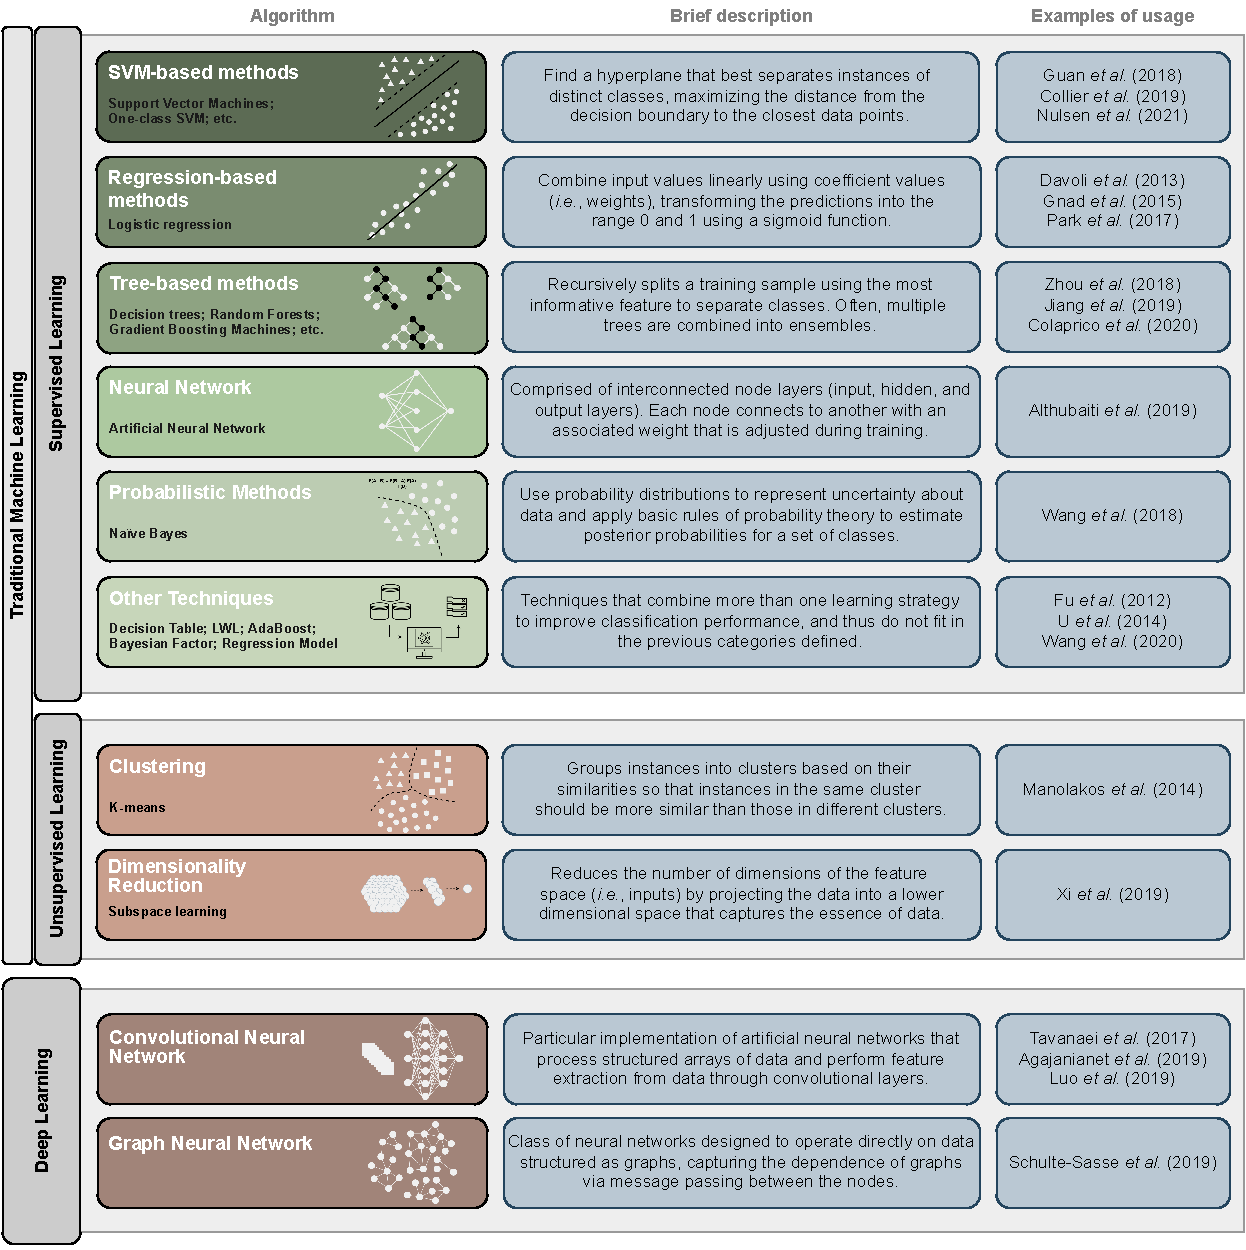
\includegraphics[width=\textwidth]{images/survey/Figure3_AlgorithmsSubcategories_Examples.pdf}
    \legend{Source: Prepared by the author}
    \label{fig:algorithm-summary}
\end{figure*}

Most papers (80\%) adopted a traditional supervised learning approach, 
exploring the known examples of true cancer drivers that are available in specialized databases (Table~\ref{tab:databases}) as training data. 
The COSMIC database \cite{cosmic} and its CGC resource \cite{sondka2018cosmic} were the most common sources for positive labels (\ie drivers), followed by TCGA (significantly mutated genes) and NCG \cite{repana2019network}. Some works restricted the selection for CDGs verified by at least two sources \cite{Colaprico2020}. High-quality negative examples (\ie non-drivers) are, in general, more challenging to define when applying ML to omics data \cite{libbrecht2015machine, schubach2017imbalance} since the choice is highly prone to biased predictions or false negatives depending on filtering criteria applied \cite{Rogers+2021}, and no comprehensive ground truth datasets are available. 
Selected papers explored mainly neutral variants from public genomic variation databases \cite{Capriotti2011, Tan2012, U2014} and synthetically generated passenger missense mutations \cite{Carter2009, Soliman2015}. Another adopted approach is to start from all genes and recursively remove positive labeled genes according to a compendium of annotation databases \cite{Schulte-Sasse2019, Wang2020}.
Many papers \cite{Soliman2015, Tokheim2016, Agajanian2018, Collier2019, Luo2019, Nicora2019, Chandrashekar2020, Colaprico2020} also collected labeled datasets from the scientific literature (\eg \cite{Carter2009, tamborero2013comprehensive, vogelstein2013cancer, martelotto2014benchmarking, bailey2018comprehensive}).

\begin{table}[!bh]
\caption{Databases adopted in the selected papers for constructing labeled datasets of positive and negative examples of cancer drivers \label{tab:databases}}
\centering
\resizebox{\linewidth}{!}{%
\begin{tabular}{L{9.2cm}|L{7.9cm}}
\hline
\multicolumn{2}{c}{\textbf{Sources for positive examples}} \\ \hline
\multicolumn{1}{l|}{\textbf{Database}} & \multicolumn{1}{l}{\textbf{References}} \\ \hline
COSMIC \cite{cosmic} or Cancer Gene Census (CGC) \cite{sondka2018cosmic} & \cite{Carter2009, Capriotti2011, Tan2012, Mao2013, Schroeder2014, U2014, Anoosha2015, Dong2016, Tavanaei2017, Jiang2019, Zhu2019, Luo2019, Colaprico2020, Chandrashekar2020, Gumpinger2020,Lyu2020} \\
TCGA  & \cite{Mao2013, Dong2016, Wang2018, Zhu2019, Chandrashekar2020, Nulsen2021} \\
Network of Cancer Genes (NCG) \cite{repana2019network} &  \cite{Schulte-Sasse2019, Cutigi2020, Nulsen2021}\\
OMIM \cite{hamosh2005online} &  \cite{Fu2012, Zhu2019}\\
intOGen \cite{gonzalez2013intogen} & \cite{Althubaiti2019, Han2019} \\
ClinVar \cite{landrum2018clinvar} &  \cite{Zhou2018}\\
CBioPortal \cite{cerami2012cbio} &\cite{Agajanian2019}\\
DriverDBv2 \cite{chung2016driverdbv2} & \cite{Han2019}\\
OncoKB \cite{chakravarty2017oncokb} & \cite{Wang2020}\\
FASMIC \cite{ng2018systematic} & \cite{Wang2020}\\\hline
\multicolumn{2}{c}{\textbf{Sources for negative examples}} \\ \hline
\multicolumn{1}{l|}{\textbf{Database}} & \multicolumn{1}{l}{\textbf{References}} \\ \hline
Synthethic examples &  \cite{Carter2009, Capriotti2011}\\
%Swiss-Prot database &  \cite{Capriotti2011}\\
Swiss-Prot Variant Pages \cite{yip2008annotating} & \cite{Capriotti2011, Tan2012} \\
CCLE \cite{barretina2012cancer} & \cite{Mao2013} \\
SNP@Domain \cite{han2006snp} &  \cite{U2014}\\
COSMIC \cite{cosmic} &  \cite{Anoosha2015}\\
%SIFT-indel & \cite{Zhou2018}\\
CBioPortal  \cite{cerami2012cbio} &\cite{Agajanian2019}\\
intOGen \cite{gonzalez2013intogen} & \cite{Althubaiti2019} \\
OncoKB \cite{chakravarty2017oncokb} & \cite{Wang2020}\\
FASMIC \cite{ng2018systematic} & \cite{Wang2020}\\
gnomAD \cite{karczewski2020mutational} & \cite{Wang2020}\\\hline
\end{tabular}%
}
\end{table}

Three papers \cite{Manolakos2014, Lu2018, Xi2019} adopted traditional unsupervised learning and four papers explored DL \cite{Tavanaei2017, Agajanian2019, Luo2019, Schulte-Sasse2019}. 

To provide a more granular discussion about traditional supervised learning approaches, we further divided them into six subcategories: SVM-based methods, regression-based methods, tree-based methods, neural network, probabilistic methods, and other approaches that do not fall into any of the previous classes. Figure~\ref{fig:Figure4_AlgorithmCategory_a} shows the algorithm categories distribution across the year of paper publication. In Figure~\ref{fig:Figure4_AlgorithmCategory_b}, we summarize the observed associations between ML strategies and data categories.

\begin{figure*}[!ht]
\centering

\caption{Analysis of types of algorithms used for model development in the selected papers. (a) Distribution of the number of occurrences found for each algorithm category per year of publication. (b) Association between data categories and algorithm categories.}

   \subfloat[\label{fig:Figure4_AlgorithmCategory_a} ]{%
      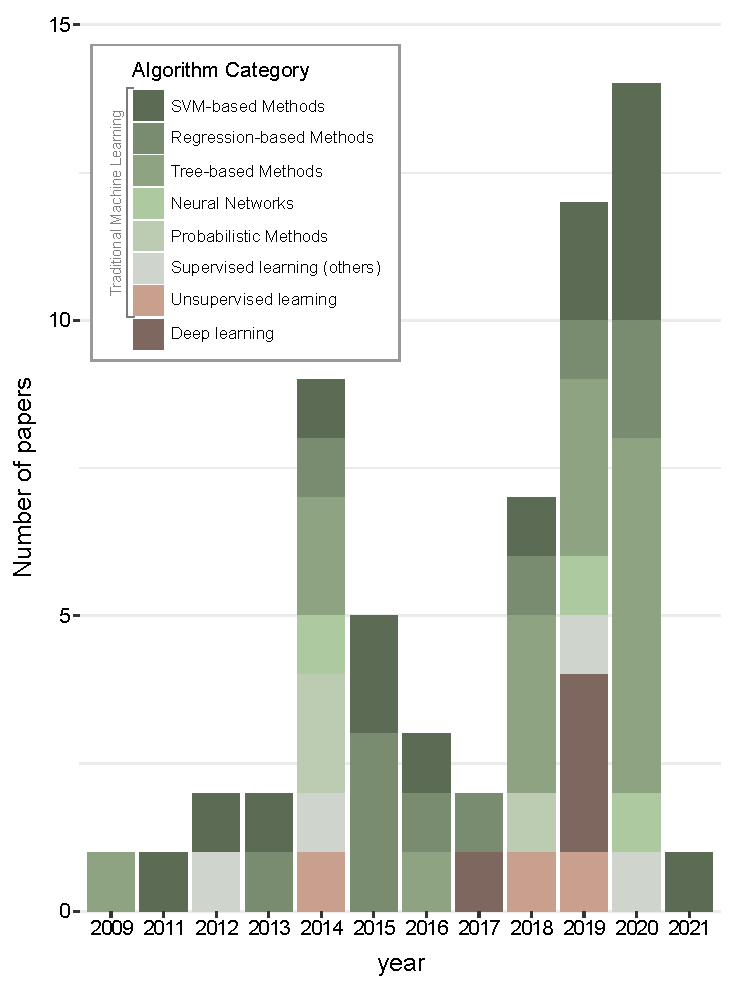
\includegraphics[width=0.52\textwidth]{images/testes/Figure4_AlgorithmCategory_a.pdf}}
\hspace{\fill}
   \subfloat[ \label{fig:Figure4_AlgorithmCategory_b}]{%
      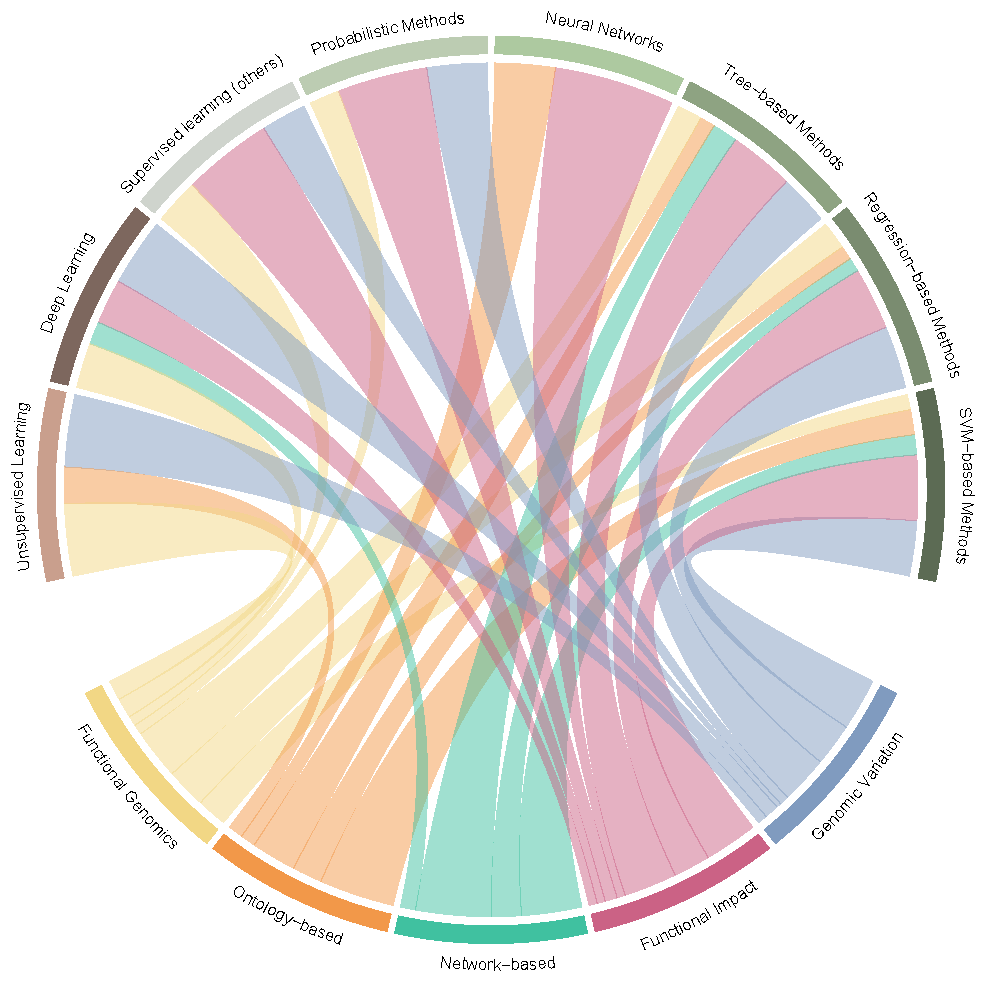
\includegraphics[width=0.63\textwidth]{images/testes/Figure4_AlgorithmCategory_b.pdf}}\\
\legend{Source: Prepared by the author}
\label{fig:algorithm-analysis}
\end{figure*}


\subsection{Methods based on traditional supervised learning}

Tree-based and SVM-based methods were the most common supervised learning approaches, observed in 39.02\% and 36.59\% of selected papers. The first proposals by \citet{Carter2009} and \citet{Capriotti2011} were based on these algorithms. Among the SVM-based approaches, whereas most papers adopted the traditional SVM algorithm \cite{Capriotti2011, Tan2012, Mao2013, U2014, Soliman2015, Dong2016, Guan2018, Cutigi2020, Gumpinger2020, Lyu2020, Wang2020}, we observed three papers using OneClass SVM \cite{Collier2019, Nicora2019, Nulsen2021} and one paper using Sequential Minimal Optimization (SMO) \cite{Anoosha2015}. SVM is a popular and consolidated technique in the field, as it continues to be largely applied since 2011.

Considering tree-based methods, although some papers explored the traditional decision tree algorithm \cite{Schroeder2014, U2014, Wang2020}, the vast majority used tree-based ensemble classifiers. Ensemble methods train multiple weak classifiers, such as decision trees, and combine their output (\eg with majority voting) to achieve a better predictive performance. We observed a frequent use of Random Forests (RF) \cite{Carter2009, Schroeder2014, U2014, Tokheim2016, Agajanian2018, Celli2018, Agajanian2019, Nicora2019, Chandrashekar2020, Colaprico2020, Cutigi2020, Gumpinger2020, Lyu2020, Wang2020}, as well as Gradient Boosting Trees (GBT) \cite{Zhou2018, Agajanian2018}, and eXtreme Gradient Boosting (XGBoost) \cite{Lyu2020, Wang2020}. Other less common tree-based variants were also explored, including Conditional trees, NB trees, and Functional trees \cite{Schroeder2014}.

Regression-based methods appeared in 11 selected papers, most of which adopted logistic regression \cite{Schroeder2014, Gnad2015, Soliman2015, Dong2016, Agajanian2018, Gumpinger2020, Lyu2020}. We also found papers using Ridge \cite{Nicora2019} and Lasso \cite{Davoli2013} regularized regressions. 

The works by Park \etal \cite{Park2015, Park2017} introduced new approaches based on linear regression and regularization schemes. Authors proposed a sparse overlapping group Lasso to perform group selection while identifying crucial genes (\ie potential CDGs) within each group \cite{Park2015}, and an interaction-based feature-selection strategy with adaptive regularization that adjusts the amount of the L1-type penalty imposed on each gene proportionally to the degree to which gene expression alteration is explained by CNAs \cite{Park2017}.


Probabilistic methods and artificial neural networks (ANN) were less frequent among selected papers. Naïve Bayes was applied in two studies \cite{Schroeder2014, U2014}, while a Bayesian network was adopted only in one \cite{U2014}. \citet{U2014} used both the traditional implementation of naïve Bayes, as well as the DTNB algorithm that combines naïve Bayes with induction of decision tables \cite{hall2008combining}. \citet{Wang2018} proposed a Bayesian hierarchical modeling approach to identify mutations that best predict alterations in gene expression, which represent candidate drivers.
Furthermore, ANNs were used in three works \cite{U2014, Althubaiti2019, Wang2020}.

\citet{Althubaiti2019} and \citet{Wang2020} trained an ANN with two hidden layers using a Rectified Linear Unit (ReLU) as an activation function for the hidden layers. In the former, the network receives as input embedding vectors generated from different ontologies, while in the latter, the input vectors are built from the pathogenicity prediction scores provided by \textit{in silico} tools.


We highlight three works that explored the greatest number of algorithms. \citet{U2014} compared 11 algorithms, including SVM-based, tree-based, ANN, and probabilistic methods. SVM presented the best performance among the classifiers, but a weighted voting approach among all models achieved the most robust results. \citet{Schroeder2014} compared six regression-based, probabilistic, and tree-based methods, and observed that RF produced the highest predictive performance. \citet{Wang2020} analyzed seven algorithms, including SVM-based, tree-based, and ANN, and pointed XGBoost as the top-performing method. 

We also identified the use of less conventional supervised learning methods, including the Bayesian Factor Regression Modeling (BFRM), a sparse statistical model for high-dimensional data analysis \cite{Fu2012}, Decision Tables, and Locally Weighted Learning (LWL) \cite{U2014}.

Finally, \citet{Han2019} applied a ML principle, but the weight parameters in the proposed score are learned by maximizing their global weighted score stats from previous genes in the training mutation data. 

\subsection{Methods based on traditional unsupervised learning}

Three papers applied unsupervised methods to CDGs prediction. \citet{Manolakos2014} proposed an algorithm for detecting gene drivers using clustering to find genes with similar expression profiles across cancer patients. Gene clusters are created using K-means, and then sparse representations of genes in a given cluster are identified as a linear combination of a small number of regulatory genes, pointed as potential cancer drivers. An Expectation-Maximization technique was used by \citet{Lu2018} in their module-based framework integrating transcriptome and genome. To identify CDGs, authors proposed an iterative approach that determines the best modulators to explain gene expression profiles of genes in a given module and re-assigns each gene to the module whose associated regulation program best predicts its behavior. In \citet{Xi2019}, a subspace learning framework was employed to obtain a low-dimensional vectorized representation of unannotated genes using a binary mutation matrix as input. Driver genes can be discriminated evaluating the distances between the output vectors and the origin in the low-dimensional subspace, with the top-ranked genes being promising driver candidates. 

\subsection{Methods based on deep learning}

Despite the increasing use of DL in Bioinformatics, only four \cite{Tavanaei2017, Agajanian2019, Luo2019, Schulte-Sasse2019} papers adopted this class of algorithms. Convolutional neural networks (CNN) were used in three papers \cite{Tavanaei2017, Agajanian2019, Luo2019} following a supervised approach. \citet{Tavanaei2017} developed a parallel CNN with three branches followed by a multi-layer fully connected neural network. Each branch receives a projection of a 3-D protein structure to a 2-D feature map set for 16 features associated with the atomic coordinates $<x, y, z>$. The input data is processed by four convolution and pooling layers adopting the ReLU activation function and three fully connected layers. \citet{Luo2019} trained a 1-D CNN with a mutation-based feature matrix as input. Authors varied the number of convolutional layers (1-4) and the number of fully connected layers (1-3), determining the best hyperparameters by grid search. 

\citet{Agajanian2019} trained a CNN model that processes encoded raw nucleotide sequences, using grid search to optimize its architecture. The authors evaluated label encoding (\ie each nucleotide receives a unique integer ID), word2vec embedding (\ie each nucleotide receives a numeric representation in a vector space based on the analysis of its sequential context), and one-hot encoding (\ie each nucleotide receives a bit encoded string), with the latter achieving best predictive performance. Their approach has the attractive property of combining high-level DNA-derived scores computed by the CNN with 32 features obtained from FI predictors as inputs for an RF model, resulting in performance improvement. 

Finally, \citet{Schulte-Sasse2019} used an extension of the CNN framework designed to handle graph-structured data as input, named Graph Convolutional Network (GCN) \cite{kipf2016semi}. The GCN directly classifies the nodes of a network based on the network structure (\eg PPI network) and nodes' characteristics (\eg gene mutation rates, gene expression, and DNA methylation) using semi-supervised learning. Their optimal GCN was composed of two graph convolutional layers with 50 and 100 filters, respectively.

\subsection{Feature selection}

Feature selection (FS) are dimensionality reduction approaches to reduce the input feature space by removing irrelevant, redundant, or noisy features, as comprehensively reviewed by \citet{li2017feature}. FS helps in decreasing the chance of overfitting, improving performance, and interpreting the patterns learned by models. Several papers explored FS in their methodology \cite{Carter2009, Tan2012, Davoli2013, Mao2013, U2014, Anoosha2015, Gnad2015, Park2015, Soliman2015, Dong2016, Park2017, Tavanaei2017, Agajanian2018, Guan2018, Zhou2018, Lyu2020, Nulsen2021}. Among these, we observed the use of mutual information \cite{Carter2009}, DX score \cite{Tan2012}, Lasso regression \cite{Davoli2013}, Mann–Whitney U test \cite{Mao2013}, and Chi-square \cite{Soliman2015}. 


\citet{U2014} applied five FS algorithms (\ie oneR, reliefF, Chi-square, gain ratio, and correlation-based) and retained all the top features indicated by at least three algorithms. \citet{Mao2013} evaluated all possible combinations with fewer than four features using k-fold cross-validation 
and the best feature subset was then expanded using a hill-climbing strategy to iteratively include the remaining features into the combination. Recursive feature elimination was employed by two papers \cite{Agajanian2018, Zhou2018}. Also, some papers analyzed feature's importance separately for oncogenes and TSGs \cite{Davoli2013, Gnad2015, Lyu2020}. \citet{Davoli2013} identified 
the LOF/benign ratio and the missense entropy as the best features to discriminate among oncogenes and TSGs in their model. 
\citet{Lyu2020} grouped correlated features using hierarchical clustering prior to FS, identifying three and five relevant feature groups for TSGs and OGs.

\subsection{Model validation protocols}

We analyzed the model validation protocols among traditional supervised learning and DL methods. This is crucial in ML methodology since an improper validation may lead to over-optimistic expectations regarding the model's performance. Two papers \cite{Tavanaei2017, Celli2018} used the basic holdout method, \ie a simple division of the original dataset into train and test sets.
A drawback of the holdout method is that the measured performance can highly depend on the instances included in the train and test datasets. \citet{Tavanaei2017} repeated the holdout process three times using different random seeds to observe performance variation; nonetheless, standard deviations were not reported. About 70.7\% of papers used the $k$-fold cross-validation process, which despite demanding more computational power and time to run, it is the most recommended approach for model validation under limited data. Besides providing a more robust performance assessment based on $k$ evaluations, it ensures that every observation from the original dataset has the chance of appearing in the train and test set. Finally, some papers \cite{Manolakos2014, Agajanian2018, Agajanian2019, Luo2019, Nicora2019} combined the holdout and the $k$-fold cross-validation methods: the k-fold cross-validation is run over the train set derived from the holdout, and the best model built during this process is further applied over the test set. This is an interesting approach, as the performance obtained for the test set is more reliable since it is guaranteed to be free from data leakage.

Additionally, some papers evaluated their predictive models with independent test sets \cite{Tan2012, Mao2013, Schroeder2014, Anoosha2015, Soliman2015, Dong2016, Tavanaei2017, Zhou2018, Collier2019, Han2019, Luo2019, Colaprico2020, Lyu2020, Wang2020, Nulsen2021}. For instance, \citet{Collier2019} used a subset of cancer genes from the Cancer Gene Census (CGC) v86 that was not included in the development of previous models. \citet{Han2019} analyzed the ability of their model to recover a set of high confidence cancer genes manually curated from literature.
\citet{Nulsen2021} evaluated their method with an independent cancer cohort data of osteosarcoma, a rare bone cancer, and found that it was able to identify reliable cancer drivers in individual patients even for cancer types not used for training. Interestingly, some papers carried out experimental analyses of selected findings to characterize mutations and their functional impact \cite{U2014, Wang2018, Han2019}.

\subsection{Predictive performance of ML strategies}

The performance of traditional supervised learning and DL methods 
was assessed mainly using accuracy, the area under the ROC curve (AUC-ROC), recall (\ie sensitivity), and precision. Some papers also summarized the trade-off between precision and recall reporting the area under the precision-recall curve (AUC-PR) and the F1-score (\ie the harmonic mean between precision and recall, attaching equal weights to both false positives and false negatives). 
Moreover, three papers reported the Matthew's Correlation Coefficient (MCC) \cite{Soliman2015, Zhou2018, Schulte-Sasse2019} and one paper \cite{Tokheim2016} proposed the mean absolute log2 fold change (MLFC) metric, which quantifies the deviation between the theoretically expected p-values and the p-values generated by a method. Although some unsupervised approaches were evaluated with the above metrics \cite{Lu2018, Xi2019}, others within this category used Jaccard index, $R^2$, and Pearson correlation \cite{Manolakos2014}.

We summarized methods' predictive performance for common metrics, as reported by the authors in their original publication (Figure \ref{fig:Perf_Analysis}). 
Since these models were evaluated on different benchmarks and for different cancer types, it is improper to compare them directly. Thus, our analysis aims to provide an overview of the predictive power achieved by ML-based methods. 
Although it may guide methodological choices in future works, it should not be used for drawing hard conclusions about top-performing approaches. Observing the trade-off between precision and recall (Figure \ref{fig:Figure5_Perf_Analysis_R2a}),  the predictive performance does not seem to be segregated by algorithm type but rather by the features type. The work by \citet{U2014} is a good example for this observation. Authors used five algorithm classes to train models with the same feature vector and found a slight variation among their performances. However, this hypothesis should be confirmed in a more profound analysis using the same experimental settings for different methods. 


\begin{figure*}[!ht]
\centering

\caption{Summary of predictive performance reported by selected papers. (a) Trade-off between precision and recall. (b) Summary of accuracy and AUC-ROC values.}

   \subfloat[ \label{fig:Figure5_Perf_Analysis_R2a} ]{%
      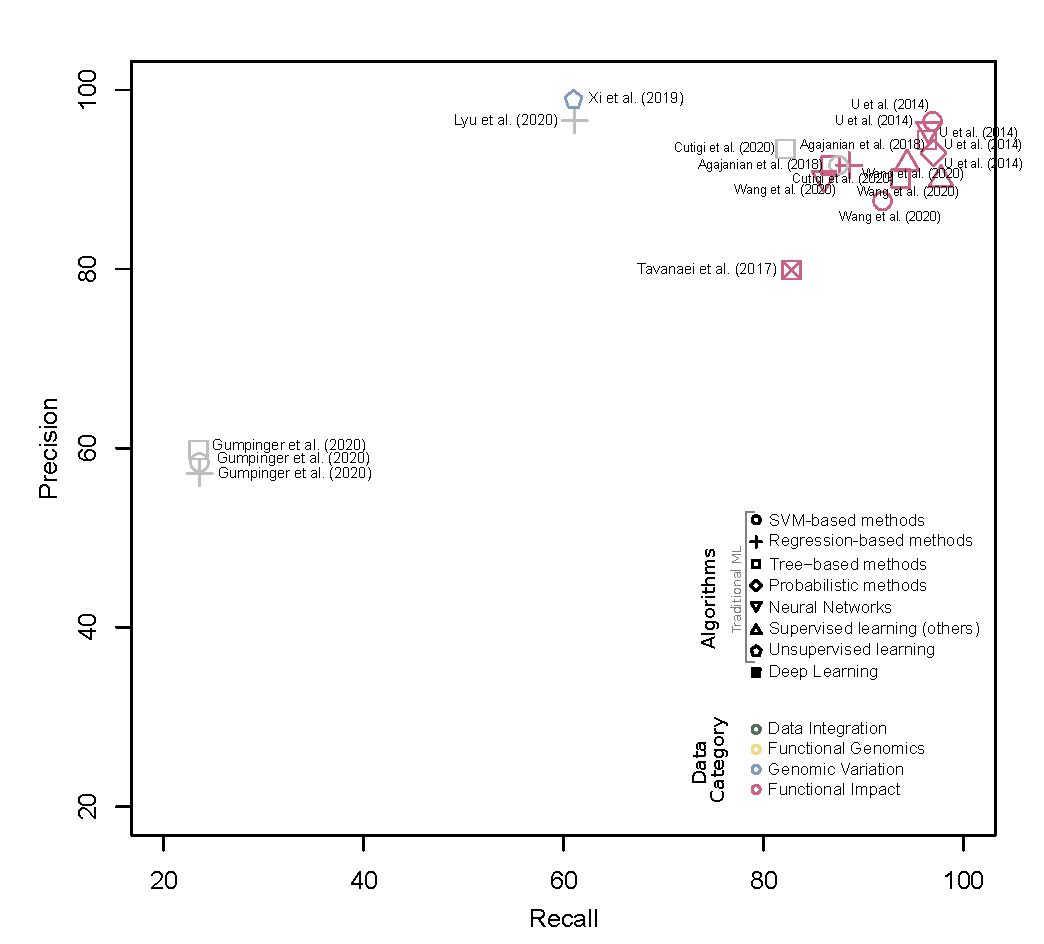
\includegraphics[width=0.68\textwidth]{images/testes/Figure5_Perf_Analysis_R2a.pdf}}
\hspace{\fill}
   \subfloat[ \label{fig:Figure5_Perf_Analysis_R2b}]{%
      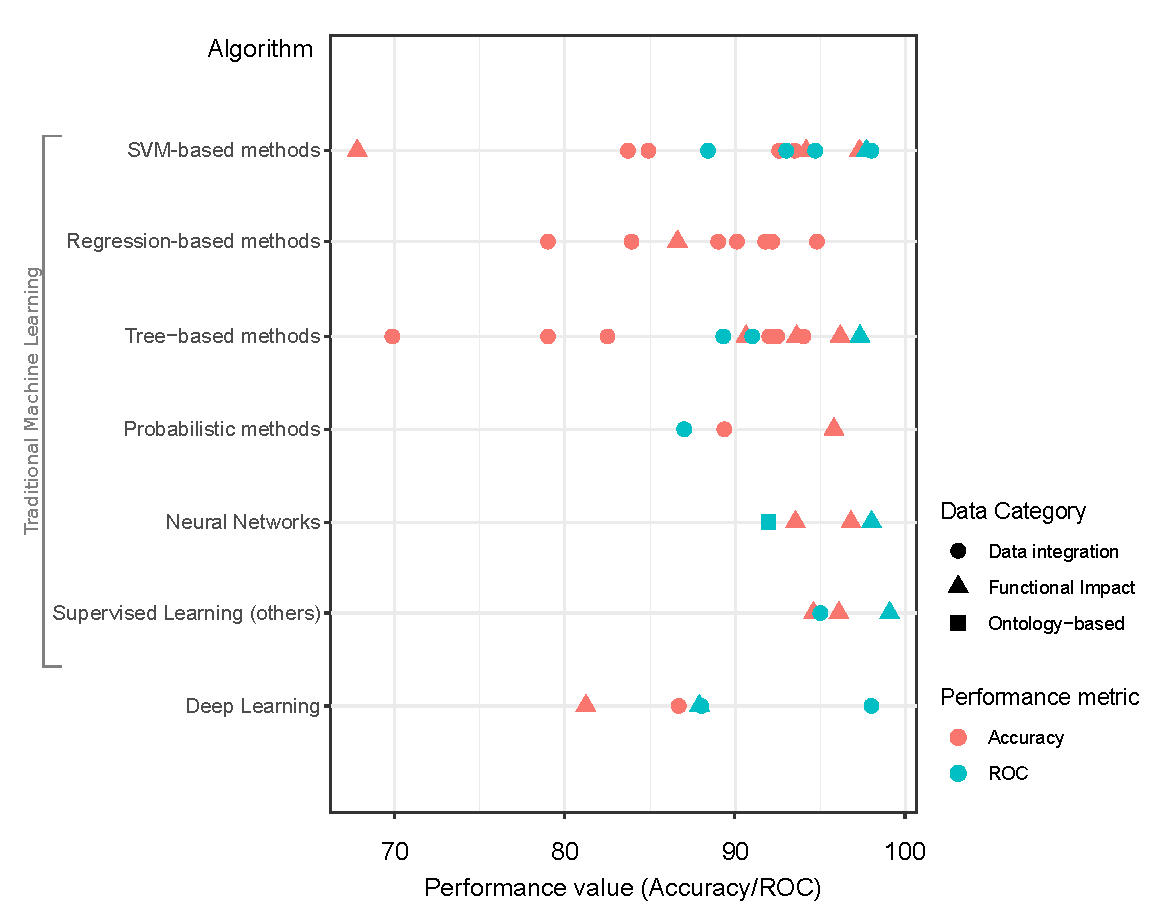
\includegraphics[width=0.73\textwidth]{images/testes/Figure5_Perf_Analysis_R2b.pdf}}\\
\legend{Source: Prepared by the author}
\label{fig:Perf_Analysis}
\end{figure*}

A summary of accuracy and AUC-ROC values (Figure~\ref{fig:Figure5_Perf_Analysis_R2b}) suggests that 
SVM-based and Tree-based methods had consistent performance, with most models surpassing the 90.00 mark. ANN and other supervised learning techniques, although not as frequent as others, also resulted in models with high predictive performance. Orienting the analysis for learning paradigms, the AUC-ROC values varied between 87.90 \cite{Tavanaei2017} and 98.00 \cite{Luo2019} for DL, and between 87.00 \cite{Wang2018} and 99.07 \cite{Wang2020} for supervised learning. The average accuracy was 89.68 and 89.90 for traditional supervised and unsupervised learning, respectively, and 83.96 for DL. However, AUC-ROC and accuracy might be deceptive and lead to incorrect conclusions with class imbalance. In general, the AUC-PR values varied from 41.65 \cite{Gumpinger2020} to 83.00 \cite{Schulte-Sasse2019}, and the F1-score from 33.40 \cite{Gumpinger2020} to 99.00 \cite{Celli2018}, reflecting a much larger variability.

Considering predictive performance, we did not observe great difference among supervised and unsupervised learning, although for the latter we only evaluated three papers. Since collecting experimentally validated driver genes may be difficult and there is currently no agreement on gold standard datasets to train and validate models \cite{raimondi2021current}, the main advantage of using unsupervised over supervised learning (either shallow or deep) is that it eliminates the need to curate positive and negative examples for training. It also alleviates the class imbalance problem and the uncertainty in the definition of non-drivers. However, as shown by \citet{Gumpinger2020}, the existing knowledge on well-established cancer genes, although limited, is valuable to improve learning results when appropriately exploited.


\section{Methodological challenges} 
\label{sec:review:challenges}

Undoubtedly, the use of ML algorithms to predict CDGs and driver mutations has enabled critical scientific advances and has an excellent potential to go even further. In this chapter, we have shed light on the broad data and algorithmic landscape behind this problem, summarizing the myriad of possibilities of combining them into novel solutions and their achievements. Nonetheless, to accelerate the computational discovery of new cancer drivers with ML, several challenges remain to be explored. In what follows, we highlight open problems identified through our review.

\subsection{Class imbalance}

The prediction of cancer driver mutations constitutes an inherent class imbalance issue, given the significantly lower number of known driver mutations in comparison to passenger mutations.
Despite the negative impact on the model development process, few selected papers using traditional supervised or deep learning approaches have discussed strategies to deal with this issue. We observed the use of undersampling of the majority class \cite{Capriotti2011, Tan2012, Gnad2015, Luo2019, Cutigi2020, Gumpinger2020}, weighted SVM \cite{Mao2013}, cost-sensitive classifier \cite{U2014}, and weighted cross-entropy as loss function \cite{Schulte-Sasse2019}. One-class SVM, although not originally designed to deal with class imbalance, may be particularly useful in this scenario \cite{Collier2019, Nulsen2021}. A better understanding of the effectiveness of existing strategies, as well as an elaboration of new ways of mitigating class imbalance, are relevant points to investigate. Semi-supervised and self-supervised learning paradigms can also be promising directions to explore.

Another related issue is the choice of appropriate performance metrics. We observed a prominent use of accuracy and AUC-ROC values for performance assessment, which under skewed class distributions do not provide adequate assessment for the minority class (\ie driver genes or mutations). Both metrics are less sensitive to false positives as the size of the negative class grows and can produce misleadingly high values. 
Thus, it is crucial to use metrics that can pay proper attention to methods' performance for the minority class, such as precision, recall, F1 score, AUC-PR, and MCC. This methodological aspect is crucial for model assessment and should not be neglected in future efforts.

\subsection{Data leakage}

Data leakage happens when information from the test set is accidentally used to develop the model.
For instance, pre-processing the complete dataset with normalization, standardization, or data imputation techniques before data partitioning causes instances from the test set to influence the train set. Similarly, performing feature selection in the complete dataset that will further be divided into independent partitions for model training and validation produces the same unintentional effect. Even under the use of cross-validation, data leakage may occur if the same test fold used to optimize the model with hyperparameter tuning or feature selection, for instance, is applied for model evaluation and selection. These methodological flaws were identified in several revised papers. Taking steps to prevent data leakage is imperative to guarantee better model generalization. Data preparation pipelines should be modeled based on training data and then applied to all partitions (\eg train, test, and validation set). 
Nested cross-validation is a promising alternative for comparing and selecting ML models with size-limited datasets, reducing the bias in the error estimate when both hyperparameter tuning and evaluation are carried out \cite{varma2006bias, vabalas2019machine}. Moreover, FS protocols designed for high-dimensional data may control optimistic performance estimates \cite{kuncheva2018feature}, especially under low-sample-size as it is the case for some cancer types.

\subsection{Data representativeness}

In ML, guaranteeing that all the variability associated with a prediction task is represented in the training dataset is as essential as data volume. In the context of cancer, the high intra- and inter-tumor heterogeneity pose additional challenges to data representativeness. Data may be unevenly distributed across distinct cancer types, tumor stages, patients' clinical profiles, or even distinct demographic groups (\eg gender and ethnicity), which certainly interferes with model generalization power. For instance, sex-associated differences in tumor molecular profiles and mutation frequency were previously reported \cite{li2018cr}. Likewise, mutational processes vary widely among cancer types \cite{brown2019finding}. Thus, any underrepresented subpopulation may suffer from biased prediction results when building models without considering this inequality. 

This rationale applies not only to a sample-oriented perspective but also to a gene-oriented perspective. Here, we highlight two possible underrepresentation issues. First, some driver genes are commonly mutated across cancer types, while others are tumor-specific \cite{poulos2019finding}. Thus, tumor-specific drivers may not be identified in pan-cancer models due to low statistical power arising from low-sample size.  Patterns from local samples tend to be diluted among patterns from the population, hindering their identification by the ML algorithm.  

Second, known cancer driver mutations tend to occur in a subset of human genes, while negative samples are spread across the genome. As discussed by \citet{raimondi2021current}, this may cause ML models to learn the simpler gene-level patterns instead of the more intricate molecular-level functional effects of driver variants, achieving an unrealistic good performance for variant-level prediction. Thus, we stress the importance of defining high-quality, unbiased negative class samples for supervised learning methods. Finally, to continue advancing, new computational strategies are needed to overcome the underrepresentation issues aforementioned. Some promising directions are developing patient-level and cohort-level methods and exploring multi-task learning for simultaneously optimizing pan-cancer and cancer-specific models. 

\subsection{Model interpretability}

Although some works have investigated the most relevant features to predict CDGs, model interpretability is still in its infancy within this domain. Model interpretability helps increase the predictive model's trust and provides valuable biological insights about molecular differences among driver and passenger mutations that may fill current knowledge gaps. Although interpreting deep learning and graph-based learning models is especially challenging, recent works have proposed strategies to comprehend the decision-making process, exploring their applications to bioinformatics \cite{schulte2021integration, talukder2021interpretation}. We advocate the use of model interpretability tools in future works as they may explain the discovered patterns and, consequently, ensure these patterns are significant and consistent with the target task (\ie avoid \textit{Clever Hans} effect \cite{lapuschkin2019unmasking}), elucidate properties associated to subgroups of drivers, and point to particular cases that deserve further attention from experts. However, we raise caution that pitfalls in model interpretability may produce incorrect conclusions \cite{molnar2020general}, thus demanding careful use.

\subsection{Non-coding drivers}

Mutations occurring in both coding and non-coding DNA regions may play a crucial role in cancer development. For instance, highly recurrent mutations in the promoter region of \textit{TERT} gene have been found in more than 50 tumor types, prompting efforts to identify additional non-coding driver events \cite{elliott2021non, bell2016understanding}. However, there are few computational tools specifically tailored for detecting drivers in non-coding regions (\eg \cite{funseq2, lawrence2013mutational, guo2020mutspot}). Identifying signals of positive selection in non-coding DNA is even more challenging because the non-coding region is about 50 times larger than the coding exome, and the number of known cancer genes with non-coding mutations is much more limited \cite{belkadi2015whole, elliott2021non}. The more frequent use of whole-genome sequencing (WGS) tends to produce more and more data that could be analyzed for this purpose. Given the several ways in which variations in non-coding DNA may contribute to tumor emergence, exploring ML learning (especially unsupervised algorithms) and the increasing volume of WGS data represents an important research opportunity to advance in the field.

\subsection{Graph-based machine learning}



Networks are pervasive in biology, representing the existing interactions between genes, gene products, and other molecules. Network-based analysis has attracted considerable attention in the prediction of disease genes in general \cite{ata2021recent}, and cancer drivers specifically \cite{zhang2016discovery, dimitrakopoulos2017computational}.
Thus, a natural and still underexplored direction in this domain is the use of graph-based ML algorithms, which can directly process graph-structured data in an end-to-end manner without the need for handcrafted feature engineering.

Graph Neural Networks (GNNs), as reviewed by \citet{wu2020comprehensive}, can better explore network's topological information for node-level or edge-level prediction tasks in contrast to traditional network analyses, thus finding several fruitful applications in Bioinformatics \cite{zhang2021graph}. Although only one selected paper adopted this approach, recent papers \cite{schulte2021integration, peng2021improving} further explored GNNs and their variants (\eg Graph Convolutional Networks) for cancer driver gene identification, obtaining outstanding performance compared with the state-of-the-art methods. 
We believe that a deeper exploration of GNNs with multimodal data (\eg multi-omics), proposing strategies to improve robustness to structural noise and class imbalance, may enable a more precise and comprehensive identification of CDGs.


\section{Summary}

In recent years, researchers have made significant progress in identifying genomic changes that contribute to the development of tumors and in distinguishing driver mutations from passenger mutations. This chapter highlights efforts that use machine learning algorithms, including traditional ML and deep learning algorithms, and summarizes the different datasets and approaches used to define features for predictive models. However, despite these advances, the field is still facing many biological and technical challenges that hinder our ability to comprehensively detect cancer drivers. To continue making progress, it is important to review significant advances and methodological details from previous research, identify gaps that need to be addressed, and propose new perspectives to advance our understanding of cancer drivers. This work focuses on one particular trend identified, which is the integration of data, and aims to address two specific challenges among those outlined in Section~\ref{sec:review:challenges}: treating class imbalance and better exploring PPI network structures during learning with graph-based learning algorithms.